\documentclass[english]{article}


\usepackage{arxiv}

\usepackage[utf8]{inputenc} % allow utf-8 input
\usepackage[T1]{fontenc}    % use 8-bit T1 fonts
\usepackage{hyperref}       % hyperlinks
\usepackage{url}            % simple URL typesetting
\usepackage{booktabs}       % professional-quality tables
\usepackage{amsfonts}       % blackboard math symbols
\usepackage{nicefrac}       % compact symbols for 1/2, etc.
\usepackage{microtype}      % microtypography
%\usepackage{lipsum}		% Can be removed after putting your text content
\usepackage{amsmath}
\usepackage{float}
\usepackage{subfigure}
\usepackage{caption}
%usepackage[demo]{graphicx}
\usepackage{nomencl}
\usepackage[figureposition=bottom,tableposition=top]{caption}
\makenomenclature
\makeindex

\usepackage{babel}

\usepackage[toc,page]{appendix}

\usepackage{tikz}
\pagestyle{empty}
\def\layersep{2.5cm}

%\setlength{\textfloatsep}{1cm}
%\setlength{\abovecaptionskip}{1cm}
%\usepackage{etoolbox}
%\BeforeBeginEnvironment{figure}{\vskip-2ex}
%\AfterEndEnvironment{figure}{\vskip-0.5ex}
%\newcommand{\squeezeup}{\vspace{-2.5mm}}


\title{Applied machine learning and deep learning to predict oil and gas production }

%\date{September 9, 1985}	% Here you can change the date presented in the paper title
%\date{} 					% Or removing it

\author{
  Luong Khanh Loc\\%\thanks{Use footnote for providing further
    %information about author (webpage, alternative
    %address)---\emph{not} for acknowledging funding agencies.} \\
  Department of Petroleum Engineerig\\
  PetroVietnam University\\
  723 CMT8, Long Toan, Baria \\
  \texttt{loclk04@pvu.edu.vn} \\
  %% examples of more authors
   \And
 Nguyen Van Hung \\
  Head of Department of Petroleum Engineering\\
  PetroVietnam University\\
  723 CMT8, Long Toan, Baria \\
  \texttt{hungnv@pvu.edu.vn} \\
  %% \AND
  %% Coauthor \\
  %% Affiliation \\
  %% Address \\
  %% \texttt{email} \\
  %% \And
  %% Coauthor \\
  %% Affiliation \\
  %% Address \\
  %% \texttt{email} \\
  %% \And
  %% Coauthor \\
  %% Affiliation \\
  %% Address \\
  %% \texttt{email} \\
}



 \usepackage{mathpazo}

    % Basic figure setup, for now with no caption control since it's done
    % automatically by Pandoc (which extracts ![](path) syntax from Markdown).
    \usepackage{graphicx}
    % We will generate all images so they have a width \maxwidth. This means
    % that they will get their normal width if they fit onto the page, but
    % are scaled down if they would overflow the margins.
    \makeatletter
    \def\maxwidth{\ifdim\Gin@nat@width>\linewidth\linewidth
    \else\Gin@nat@width\fi}
    \makeatother
    \let\Oldincludegraphics\includegraphics
    % Set max figure width to be 80% of text width, for now hardcoded.
    \renewcommand{\includegraphics}[1]{\Oldincludegraphics[width=.8\maxwidth]{#1}}
    % Ensure that by default, figures have no caption (until we provide a
    % proper Figure object with a Caption API and a way to capture that
    % in the conversion process - todo).
    \usepackage{caption}
    \DeclareCaptionLabelFormat{nolabel}{}
    \captionsetup{labelformat=nolabel}

    \usepackage{adjustbox} % Used to constrain images to a maximum size 
    \usepackage{xcolor} % Allow colors to be defined
    \usepackage{enumerate} % Needed for markdown enumerations to work
    \usepackage{geometry} % Used to adjust the document margins
    \usepackage{amsmath} % Equations
    \usepackage{amssymb} % Equations
    \usepackage{textcomp} % defines textquotesingle
    % Hack from http://tex.stackexchange.com/a/47451/13684:
    \AtBeginDocument{%
        \def\PYZsq{\textquotesingle}% Upright quotes in Pygmentized code
    }
    \usepackage{upquote} % Upright quotes for verbatim code
    \usepackage{eurosym} % defines \euro
    \usepackage[mathletters]{ucs} % Extended unicode (utf-8) support
    \usepackage[utf8x]{inputenc} % Allow utf-8 characters in the tex document
    \usepackage{fancyvrb} % verbatim replacement that allows latex
    \usepackage{grffile} % extends the file name processing of package graphics 
                         % to support a larger range 
    % The hyperref package gives us a pdf with properly built
    % internal navigation ('pdf bookmarks' for the table of contents,
    % internal cross-reference links, web links for URLs, etc.)
    \usepackage{hyperref}
    \usepackage{longtable} % longtable support required by pandoc >1.10
    \usepackage{booktabs}  % table support for pandoc > 1.12.2
    \usepackage[inline]{enumitem} % IRkernel/repr support (it uses the enumerate* environment)
    \usepackage[normalem]{ulem} % ulem is needed to support strikethroughs (\sout)
                                % normalem makes italics be italics, not underlines
    \usepackage{mathrsfs}
    

    
    
    % Colors for the hyperref package
    \definecolor{urlcolor}{rgb}{0,.145,.698}
    \definecolor{linkcolor}{rgb}{.71,0.21,0.01}
    \definecolor{citecolor}{rgb}{.12,.54,.11}

    % ANSI colors
    \definecolor{ansi-black}{HTML}{3E424D}
    \definecolor{ansi-black-intense}{HTML}{282C36}
    \definecolor{ansi-red}{HTML}{E75C58}
    \definecolor{ansi-red-intense}{HTML}{B22B31}
    \definecolor{ansi-green}{HTML}{00A250}
    \definecolor{ansi-green-intense}{HTML}{007427}
    \definecolor{ansi-yellow}{HTML}{DDB62B}
    \definecolor{ansi-yellow-intense}{HTML}{B27D12}
    \definecolor{ansi-blue}{HTML}{208FFB}
    \definecolor{ansi-blue-intense}{HTML}{0065CA}
    \definecolor{ansi-magenta}{HTML}{D160C4}
    \definecolor{ansi-magenta-intense}{HTML}{A03196}
    \definecolor{ansi-cyan}{HTML}{60C6C8}
    \definecolor{ansi-cyan-intense}{HTML}{258F8F}
    \definecolor{ansi-white}{HTML}{C5C1B4}
    \definecolor{ansi-white-intense}{HTML}{A1A6B2}
    \definecolor{ansi-default-inverse-fg}{HTML}{FFFFFF}
    \definecolor{ansi-default-inverse-bg}{HTML}{000000}

    % commands and environments needed by pandoc snippets
    % extracted from the output of `pandoc -s`
    \providecommand{\tightlist}{%
      \setlength{\itemsep}{0pt}\setlength{\parskip}{0pt}}
    \DefineVerbatimEnvironment{Highlighting}{Verbatim}{commandchars=\\\{\}}
    % Add ',fontsize=\small' for more characters per line
    \newenvironment{Shaded}{}{}
    \newcommand{\KeywordTok}[1]{\textcolor[rgb]{0.00,0.44,0.13}{\textbf{{#1}}}}
    \newcommand{\DataTypeTok}[1]{\textcolor[rgb]{0.56,0.13,0.00}{{#1}}}
    \newcommand{\DecValTok}[1]{\textcolor[rgb]{0.25,0.63,0.44}{{#1}}}
    \newcommand{\BaseNTok}[1]{\textcolor[rgb]{0.25,0.63,0.44}{{#1}}}
    \newcommand{\FloatTok}[1]{\textcolor[rgb]{0.25,0.63,0.44}{{#1}}}
    \newcommand{\CharTok}[1]{\textcolor[rgb]{0.25,0.44,0.63}{{#1}}}
    \newcommand{\StringTok}[1]{\textcolor[rgb]{0.25,0.44,0.63}{{#1}}}
    \newcommand{\CommentTok}[1]{\textcolor[rgb]{0.38,0.63,0.69}{\textit{{#1}}}}
    \newcommand{\OtherTok}[1]{\textcolor[rgb]{0.00,0.44,0.13}{{#1}}}
    \newcommand{\AlertTok}[1]{\textcolor[rgb]{1.00,0.00,0.00}{\textbf{{#1}}}}
    \newcommand{\FunctionTok}[1]{\textcolor[rgb]{0.02,0.16,0.49}{{#1}}}
    \newcommand{\RegionMarkerTok}[1]{{#1}}
    \newcommand{\ErrorTok}[1]{\textcolor[rgb]{1.00,0.00,0.00}{\textbf{{#1}}}}
    \newcommand{\NormalTok}[1]{{#1}}
    
    % Additional commands for more recent versions of Pandoc
    \newcommand{\ConstantTok}[1]{\textcolor[rgb]{0.53,0.00,0.00}{{#1}}}
    \newcommand{\SpecialCharTok}[1]{\textcolor[rgb]{0.25,0.44,0.63}{{#1}}}
    \newcommand{\VerbatimStringTok}[1]{\textcolor[rgb]{0.25,0.44,0.63}{{#1}}}
    \newcommand{\SpecialStringTok}[1]{\textcolor[rgb]{0.73,0.40,0.53}{{#1}}}
    \newcommand{\ImportTok}[1]{{#1}}
    \newcommand{\DocumentationTok}[1]{\textcolor[rgb]{0.73,0.13,0.13}{\textit{{#1}}}}
    \newcommand{\AnnotationTok}[1]{\textcolor[rgb]{0.38,0.63,0.69}{\textbf{\textit{{#1}}}}}
    \newcommand{\CommentVarTok}[1]{\textcolor[rgb]{0.38,0.63,0.69}{\textbf{\textit{{#1}}}}}
    \newcommand{\VariableTok}[1]{\textcolor[rgb]{0.10,0.09,0.49}{{#1}}}
    \newcommand{\ControlFlowTok}[1]{\textcolor[rgb]{0.00,0.44,0.13}{\textbf{{#1}}}}
    \newcommand{\OperatorTok}[1]{\textcolor[rgb]{0.40,0.40,0.40}{{#1}}}
    \newcommand{\BuiltInTok}[1]{{#1}}
    \newcommand{\ExtensionTok}[1]{{#1}}
    \newcommand{\PreprocessorTok}[1]{\textcolor[rgb]{0.74,0.48,0.00}{{#1}}}
    \newcommand{\AttributeTok}[1]{\textcolor[rgb]{0.49,0.56,0.16}{{#1}}}
    \newcommand{\InformationTok}[1]{\textcolor[rgb]{0.38,0.63,0.69}{\textbf{\textit{{#1}}}}}
    \newcommand{\WarningTok}[1]{\textcolor[rgb]{0.38,0.63,0.69}{\textbf{\textit{{#1}}}}}
    
    
    % Define a nice break command that doesn't care if a line doesn't already
    % exist.
    \def\br{\hspace*{\fill} \\* }
    % Math Jax compatibility definitions
    \def\gt{>}
    \def\lt{<}
    \let\Oldtex\TeX
    \let\Oldlatex\LaTeX
    \renewcommand{\TeX}{\textrm{\Oldtex}}
    \renewcommand{\LaTeX}{\textrm{\Oldlatex}}
    % Document parameters
    % Document title
    \title{Untitled1}
    
    
    
    
    

    % Pygments definitions
    
\makeatletter
\def\PY@reset{\let\PY@it=\relax \let\PY@bf=\relax%
    \let\PY@ul=\relax \let\PY@tc=\relax%
    \let\PY@bc=\relax \let\PY@ff=\relax}
\def\PY@tok#1{\csname PY@tok@#1\endcsname}
\def\PY@toks#1+{\ifx\relax#1\empty\else%
    \PY@tok{#1}\expandafter\PY@toks\fi}
\def\PY@do#1{\PY@bc{\PY@tc{\PY@ul{%
    \PY@it{\PY@bf{\PY@ff{#1}}}}}}}
\def\PY#1#2{\PY@reset\PY@toks#1+\relax+\PY@do{#2}}

\expandafter\def\csname PY@tok@w\endcsname{\def\PY@tc##1{\textcolor[rgb]{0.73,0.73,0.73}{##1}}}
\expandafter\def\csname PY@tok@c\endcsname{\let\PY@it=\textit\def\PY@tc##1{\textcolor[rgb]{0.25,0.50,0.50}{##1}}}
\expandafter\def\csname PY@tok@cp\endcsname{\def\PY@tc##1{\textcolor[rgb]{0.74,0.48,0.00}{##1}}}
\expandafter\def\csname PY@tok@k\endcsname{\let\PY@bf=\textbf\def\PY@tc##1{\textcolor[rgb]{0.00,0.50,0.00}{##1}}}
\expandafter\def\csname PY@tok@kp\endcsname{\def\PY@tc##1{\textcolor[rgb]{0.00,0.50,0.00}{##1}}}
\expandafter\def\csname PY@tok@kt\endcsname{\def\PY@tc##1{\textcolor[rgb]{0.69,0.00,0.25}{##1}}}
\expandafter\def\csname PY@tok@o\endcsname{\def\PY@tc##1{\textcolor[rgb]{0.40,0.40,0.40}{##1}}}
\expandafter\def\csname PY@tok@ow\endcsname{\let\PY@bf=\textbf\def\PY@tc##1{\textcolor[rgb]{0.67,0.13,1.00}{##1}}}
\expandafter\def\csname PY@tok@nb\endcsname{\def\PY@tc##1{\textcolor[rgb]{0.00,0.50,0.00}{##1}}}
\expandafter\def\csname PY@tok@nf\endcsname{\def\PY@tc##1{\textcolor[rgb]{0.00,0.00,1.00}{##1}}}
\expandafter\def\csname PY@tok@nc\endcsname{\let\PY@bf=\textbf\def\PY@tc##1{\textcolor[rgb]{0.00,0.00,1.00}{##1}}}
\expandafter\def\csname PY@tok@nn\endcsname{\let\PY@bf=\textbf\def\PY@tc##1{\textcolor[rgb]{0.00,0.00,1.00}{##1}}}
\expandafter\def\csname PY@tok@ne\endcsname{\let\PY@bf=\textbf\def\PY@tc##1{\textcolor[rgb]{0.82,0.25,0.23}{##1}}}
\expandafter\def\csname PY@tok@nv\endcsname{\def\PY@tc##1{\textcolor[rgb]{0.10,0.09,0.49}{##1}}}
\expandafter\def\csname PY@tok@no\endcsname{\def\PY@tc##1{\textcolor[rgb]{0.53,0.00,0.00}{##1}}}
\expandafter\def\csname PY@tok@nl\endcsname{\def\PY@tc##1{\textcolor[rgb]{0.63,0.63,0.00}{##1}}}
\expandafter\def\csname PY@tok@ni\endcsname{\let\PY@bf=\textbf\def\PY@tc##1{\textcolor[rgb]{0.60,0.60,0.60}{##1}}}
\expandafter\def\csname PY@tok@na\endcsname{\def\PY@tc##1{\textcolor[rgb]{0.49,0.56,0.16}{##1}}}
\expandafter\def\csname PY@tok@nt\endcsname{\let\PY@bf=\textbf\def\PY@tc##1{\textcolor[rgb]{0.00,0.50,0.00}{##1}}}
\expandafter\def\csname PY@tok@nd\endcsname{\def\PY@tc##1{\textcolor[rgb]{0.67,0.13,1.00}{##1}}}
\expandafter\def\csname PY@tok@s\endcsname{\def\PY@tc##1{\textcolor[rgb]{0.73,0.13,0.13}{##1}}}
\expandafter\def\csname PY@tok@sd\endcsname{\let\PY@it=\textit\def\PY@tc##1{\textcolor[rgb]{0.73,0.13,0.13}{##1}}}
\expandafter\def\csname PY@tok@si\endcsname{\let\PY@bf=\textbf\def\PY@tc##1{\textcolor[rgb]{0.73,0.40,0.53}{##1}}}
\expandafter\def\csname PY@tok@se\endcsname{\let\PY@bf=\textbf\def\PY@tc##1{\textcolor[rgb]{0.73,0.40,0.13}{##1}}}
\expandafter\def\csname PY@tok@sr\endcsname{\def\PY@tc##1{\textcolor[rgb]{0.73,0.40,0.53}{##1}}}
\expandafter\def\csname PY@tok@ss\endcsname{\def\PY@tc##1{\textcolor[rgb]{0.10,0.09,0.49}{##1}}}
\expandafter\def\csname PY@tok@sx\endcsname{\def\PY@tc##1{\textcolor[rgb]{0.00,0.50,0.00}{##1}}}
\expandafter\def\csname PY@tok@m\endcsname{\def\PY@tc##1{\textcolor[rgb]{0.40,0.40,0.40}{##1}}}
\expandafter\def\csname PY@tok@gh\endcsname{\let\PY@bf=\textbf\def\PY@tc##1{\textcolor[rgb]{0.00,0.00,0.50}{##1}}}
\expandafter\def\csname PY@tok@gu\endcsname{\let\PY@bf=\textbf\def\PY@tc##1{\textcolor[rgb]{0.50,0.00,0.50}{##1}}}
\expandafter\def\csname PY@tok@gd\endcsname{\def\PY@tc##1{\textcolor[rgb]{0.63,0.00,0.00}{##1}}}
\expandafter\def\csname PY@tok@gi\endcsname{\def\PY@tc##1{\textcolor[rgb]{0.00,0.63,0.00}{##1}}}
\expandafter\def\csname PY@tok@gr\endcsname{\def\PY@tc##1{\textcolor[rgb]{1.00,0.00,0.00}{##1}}}
\expandafter\def\csname PY@tok@ge\endcsname{\let\PY@it=\textit}
\expandafter\def\csname PY@tok@gs\endcsname{\let\PY@bf=\textbf}
\expandafter\def\csname PY@tok@gp\endcsname{\let\PY@bf=\textbf\def\PY@tc##1{\textcolor[rgb]{0.00,0.00,0.50}{##1}}}
\expandafter\def\csname PY@tok@go\endcsname{\def\PY@tc##1{\textcolor[rgb]{0.53,0.53,0.53}{##1}}}
\expandafter\def\csname PY@tok@gt\endcsname{\def\PY@tc##1{\textcolor[rgb]{0.00,0.27,0.87}{##1}}}
\expandafter\def\csname PY@tok@err\endcsname{\def\PY@bc##1{\setlength{\fboxsep}{0pt}\fcolorbox[rgb]{1.00,0.00,0.00}{1,1,1}{\strut ##1}}}
\expandafter\def\csname PY@tok@kc\endcsname{\let\PY@bf=\textbf\def\PY@tc##1{\textcolor[rgb]{0.00,0.50,0.00}{##1}}}
\expandafter\def\csname PY@tok@kd\endcsname{\let\PY@bf=\textbf\def\PY@tc##1{\textcolor[rgb]{0.00,0.50,0.00}{##1}}}
\expandafter\def\csname PY@tok@kn\endcsname{\let\PY@bf=\textbf\def\PY@tc##1{\textcolor[rgb]{0.00,0.50,0.00}{##1}}}
\expandafter\def\csname PY@tok@kr\endcsname{\let\PY@bf=\textbf\def\PY@tc##1{\textcolor[rgb]{0.00,0.50,0.00}{##1}}}
\expandafter\def\csname PY@tok@bp\endcsname{\def\PY@tc##1{\textcolor[rgb]{0.00,0.50,0.00}{##1}}}
\expandafter\def\csname PY@tok@fm\endcsname{\def\PY@tc##1{\textcolor[rgb]{0.00,0.00,1.00}{##1}}}
\expandafter\def\csname PY@tok@vc\endcsname{\def\PY@tc##1{\textcolor[rgb]{0.10,0.09,0.49}{##1}}}
\expandafter\def\csname PY@tok@vg\endcsname{\def\PY@tc##1{\textcolor[rgb]{0.10,0.09,0.49}{##1}}}
\expandafter\def\csname PY@tok@vi\endcsname{\def\PY@tc##1{\textcolor[rgb]{0.10,0.09,0.49}{##1}}}
\expandafter\def\csname PY@tok@vm\endcsname{\def\PY@tc##1{\textcolor[rgb]{0.10,0.09,0.49}{##1}}}
\expandafter\def\csname PY@tok@sa\endcsname{\def\PY@tc##1{\textcolor[rgb]{0.73,0.13,0.13}{##1}}}
\expandafter\def\csname PY@tok@sb\endcsname{\def\PY@tc##1{\textcolor[rgb]{0.73,0.13,0.13}{##1}}}
\expandafter\def\csname PY@tok@sc\endcsname{\def\PY@tc##1{\textcolor[rgb]{0.73,0.13,0.13}{##1}}}
\expandafter\def\csname PY@tok@dl\endcsname{\def\PY@tc##1{\textcolor[rgb]{0.73,0.13,0.13}{##1}}}
\expandafter\def\csname PY@tok@s2\endcsname{\def\PY@tc##1{\textcolor[rgb]{0.73,0.13,0.13}{##1}}}
\expandafter\def\csname PY@tok@sh\endcsname{\def\PY@tc##1{\textcolor[rgb]{0.73,0.13,0.13}{##1}}}
\expandafter\def\csname PY@tok@s1\endcsname{\def\PY@tc##1{\textcolor[rgb]{0.73,0.13,0.13}{##1}}}
\expandafter\def\csname PY@tok@mb\endcsname{\def\PY@tc##1{\textcolor[rgb]{0.40,0.40,0.40}{##1}}}
\expandafter\def\csname PY@tok@mf\endcsname{\def\PY@tc##1{\textcolor[rgb]{0.40,0.40,0.40}{##1}}}
\expandafter\def\csname PY@tok@mh\endcsname{\def\PY@tc##1{\textcolor[rgb]{0.40,0.40,0.40}{##1}}}
\expandafter\def\csname PY@tok@mi\endcsname{\def\PY@tc##1{\textcolor[rgb]{0.40,0.40,0.40}{##1}}}
\expandafter\def\csname PY@tok@il\endcsname{\def\PY@tc##1{\textcolor[rgb]{0.40,0.40,0.40}{##1}}}
\expandafter\def\csname PY@tok@mo\endcsname{\def\PY@tc##1{\textcolor[rgb]{0.40,0.40,0.40}{##1}}}
\expandafter\def\csname PY@tok@ch\endcsname{\let\PY@it=\textit\def\PY@tc##1{\textcolor[rgb]{0.25,0.50,0.50}{##1}}}
\expandafter\def\csname PY@tok@cm\endcsname{\let\PY@it=\textit\def\PY@tc##1{\textcolor[rgb]{0.25,0.50,0.50}{##1}}}
\expandafter\def\csname PY@tok@cpf\endcsname{\let\PY@it=\textit\def\PY@tc##1{\textcolor[rgb]{0.25,0.50,0.50}{##1}}}
\expandafter\def\csname PY@tok@c1\endcsname{\let\PY@it=\textit\def\PY@tc##1{\textcolor[rgb]{0.25,0.50,0.50}{##1}}}
\expandafter\def\csname PY@tok@cs\endcsname{\let\PY@it=\textit\def\PY@tc##1{\textcolor[rgb]{0.25,0.50,0.50}{##1}}}

\def\PYZbs{\char`\\}
\def\PYZus{\char`\_}
\def\PYZob{\char`\{}
\def\PYZcb{\char`\}}
\def\PYZca{\char`\^}
\def\PYZam{\char`\&}
\def\PYZlt{\char`\<}
\def\PYZgt{\char`\>}
\def\PYZsh{\char`\#}
\def\PYZpc{\char`\%}
\def\PYZdl{\char`\$}
\def\PYZhy{\char`\-}
\def\PYZsq{\char`\'}
\def\PYZdq{\char`\"}
\def\PYZti{\char`\~}
% for compatibility with earlier versions
\def\PYZat{@}
\def\PYZlb{[}
\def\PYZrb{]}
\makeatother


    % Exact colors from NB
    \definecolor{incolor}{rgb}{0.0, 0.0, 0.5}
    \definecolor{outcolor}{rgb}{0.545, 0.0, 0.0}



    
    % Prevent overflowing lines due to hard-to-break entities
    \sloppy 
    % Setup hyperref package
    \hypersetup{
      breaklinks=true,  % so long urls are correctly broken across lines
      colorlinks=true,
      urlcolor=urlcolor,
      linkcolor=linkcolor,
      citecolor=citecolor,
      }



\begin{document}
\maketitle

\begin{abstract}
%\lipsum[1]
Recently, artificial intelligent (AI) has gained a great deal of attention in many areas, especially oil and gas industry. There was a significant development of AI that enables oil and gas companies to reduce a huge amount of cost and make more accurate decisions. In this paper, a new method based on Artificial Intelligence including machine learning and deep learning techniques has applied to petroleum engineering to predict the oil and gas production.\\
Bottom hole pressure and flow rate are predicted using various algorithms based on AI technique. This study proposed a novel approach using Regression algorithms and Ensemble methods to leverage the results. A  typical Recurrent Neural Networks include Long Short Term Memory (LSTM), Gated Recurrent Unit (GRU) and Simple RNN has been developed to predict oil ans gas production. \\
This research focuses on figuring out the potential and efficiency of machine learning and deep learning algorithms to predict production in the future. This study explored ten different machine/deep learning algorithms and their performance evaluation.Python is choosen for this purposes because of its useful and robust machine/deep learning libraries.
\end{abstract}


% keywords can be removed
\keywords{machine learning \and deep learning \and production forecasting \and artificial intelligent \and volve dataset}


%\section{Abstract}
%\lipsum[2]
%\lipsum[3]


\section{Introduction}
\label{sec:headings}
Artificial Intelligence (AI) is transforming the oil and gas industry. A study from McKinsey (2016) in 2016 mentioned that digital organization, which covers AI and Machine Learning, is one of the five big ideas that will reshape the future of the industry. Digitizing and automating work will result in better safety and productivity as fewer people will be at risk and the risk of human error is reduced. Moreover, in the low oil price environment, oil companies often have no choice but to cut their operational budget, reduce the headcount, and/or fully optimize their remaining assets. This further encourages the adoption of artificial intelligence in the industry, with the hope to simplify and/or automate inefficient processes.\cite{Ristanto}.\\
%\lipsum[4] See Section \ref{sec:headings}.

There have been some implementations of AI in the field of oil and gas production. Boomer (1995) \cite{Boomer}used Neural Network to forecast oil production in Vacuum Field, Texas and the model outperformed the professionals 93\% of the time. Cao et al. (2016) found that Neural Network performed better than conventional decline curve methods (Arps, Duong, and Stretched Exponential Production Decline). Suhag et al. (2017) \cite{Suhag} implemented Neural Network to predict oil rate in Bakken shale wells and yielded better results than Duong’s method. J. Sun, X. Ma, and M. Kazi \cite{Sun} have recently propose a novel method of using Recurrent Neural Networks for production forecast and it give outperformed results compared to conventional methods like DCA, SEPD and Duong.\\

In this paper, we have develop a workflow of using machine learning and deep learning techique to predict future production rate. Ensemble methods have been built to gain better result. We also used three kind of Recurrent Neural Network for prediction.

\section{Artificial Intelligence}
Artificial intelligence is a branch of computer science that aims to create intelligent machines. It has become an essential part of the technology industry. Artificial intelligence (AI) is the simulation of human intelligence processes by machines, especially computer systems. These processes include learning (the acquisition of information and rules for using the information), reasoning (using rules to reach approximate or definite conclusions) and self-correction. Particular applications of AI include expert systems, speech recognition and machine vision.\\
Machine learning and deep learning are core part of AI. Learning without any kind of supervision requires an ability to identify patterns in streams of inputs, whereas learning with adequate supervision involves classification and numerical regressions. Classification determines the category an object belongs to and regression deals with obtaining a set of numerical input or output examples, thereby discovering functions enabling the generation of suitable outputs from respective inputs.\\

\subsection{Machine learning}
Machine learning is a statistical technology to get computers output expected results without being explicitly programmed. Machine learning is based on big-data without explicitly programming, therefore, it saves programming time and avoids various ideal scenarios restrictions, and it also improves the output prediction accuracy. Machine learning method such as Artificial Neural Network (ANN) is applied in oil and gas industry for production forecasting \cite{Cao}(Cao et al., 2016).\\
The main objective of every machine learning algorithms is to find a optimal set of parameters $\mathbb{w}$ tailoring of the hypothesis to a specific set of data.
In this paper, we have used 12 different machine learning algorithms for prediction. A brief overview of 12 algorithms we have used will be introduced below.
\subsubsection{Linear Regression}
The simplest linear model for regression is one that involves a linear combination of
the input variables\cite{Bishop}
\begin{equation}
y(\textbf{x}, \textbf{w}) = w_{0} w_{1}x_{1} + \ldots + w_{D}x_{D} 
\end{equation}
where $x = (x_{1},\ldots,x_{D})^{T}$.The key property of this model is that it is a linear function of the parameters $w_{0} , \ldots, w_{D}$. It is also, however, a linear function of the input variables xi, and this imposes significant limitations on the model. We therefore extend the class of models by considering linear combinations of fixed nonlinear functions of the input variables, of the form:
\begin{equation}
y(\textbf{x}, \textbf{w}) =  w_{0} + \sum_{j=1}^{M-1} w_{j}\phi_{j}(x)
\end{equation}
where $\phi_{j} (x)$are known as basis functions.\\
In this research, we just applied linear regression as the simplest model of machine learning algotithms for prediction.
\subsubsection{Ridge}
Rigde is a Linear least squares with L2 regularization. Ridge regression addresses some of the problems of Ordinary Least Squares by imposing a penalty on the size of coefficients. The ridge coefficients minimize a penalized residual sum of squares.\cite{sklearn}
\begin{equation}
\min_{w} = \parallel Xw - y \parallel_{2}^2 +\alpha\parallel w \parallel_{2}^2
\end{equation}
Here,$\alpha \ge 0 $ is a complexity parameter that controls the amount of shrinkage: the larger the value of $\alpha$, the greater the amount of shrinkage and thus the coefficients become more robust to collinearity.
\subsubsection{KNeighbors Regression}
K-Nearest Neighbors uses local neighborhood points to make a prediction. In more detail, distance (Euclidean distance in this study) is calculated from a query point $x^{(i)}$ in the test set to each data point $x^{'(i)}$ in the training time:
\begin{equation}
D(x,x^{'}) = \sqrt{\sum_{i=1}^{N}(x^{(i)} - x^{'(i)})^{2}}
\end{equation}
Continuousky, sorting the distance and pick k closest data points. Define the k points closest points in the training set that are closest to x the set G. The prediction during testing time is calculated by local interpolation of the nearest neighbors in G \cite{Ristanto}.
\begin{equation}
\hat{y}^{i} = \frac{1}{K} \sum_{j\in G}^{N} y_{j}
\end{equation}
where $\hat{y}^{i}$ is the output of KNeighbors regressor and k is the number of nearest neighbors points.
\subsubsection{Support Vector Regression}
The method of Support Vector Regression is extended from SVM algorithms to solve the regression problems.\\
Given training vectors $x_{i} \in \mathbb{R}^{p}, i = 1, \ldots, n$ and a vector $y \in \mathbb{R}^{n}$, SVR solves the following primal problem:
\begin{equation}
\min_{w,b,\zeta,\zeta^{\ast}} \frac{1}{2}w^{T}w + C\sum_{i=1}^{n}(\zeta_{i} + \zeta_{i}^{\ast})
\end{equation}
\begin{align*}
subject\,to\,: y_{i} - w^{T}\phi(x_{i}) - b \leq \varepsilon + \zeta_{i}^{\ast},\\
w^{T}\phi(x_{i}) + b - y_{i} \leq \varepsilon + \zeta_{i}^{\ast},\\
\zeta_{i},\zeta_{i}^{\ast} \geq 0, i = 1,\ldots,n.
\end{align*}
\subsubsection{Decision Tree Regression}
Decision Tree \cite{Dom} (also called Regression Tree in regression problems) is a supervised learning model that creates branches of decision nodes. Decision Tree learns a dataset by making the best split of features in the training set into subsets based on the homogeneity of each new subset. The process goes on until a stopping criterion (e.g. tree size or number of observation per node) is reached (Breiman et al. 1984).\\
Data $y \in \mathbb{R}^{n}, X \in \mathbb{R}^{n\times p}$ and observation $(y_{i},x_{i}) \in \mathbb{R}^{p+1}, i = 1,\ldots,n.$
Suppose we have a partition of $R^{p}$ into M regions $R_{1}, \ldots, R_{m}$.We predict the response using a constant on each $R_{i}$:
\begin{equation}
f(x) = \sum_{i=1}^{m}c_{i}\cdot \textbf{1}_{x_{i} \in \mathbb{R}_{i}}
\end{equation}
In order to optimize $\sum_{i=1}^{n}(y_{i} - f(x_{i}))^2$, one needs to choose: $\hat{c}_{i} = ave(y_{j}: x_{j} \in \mathbb{R}_{i})$.\\
Consider a splitting variable $j \in {1, \ldots, p} $and splitting point $s \in \mathbb{R}$. Define the two half-plane:
\begin{align*}
R_{1}(j,s) := \{x \in \mathbb{R}^{p}: x_{j} \leq s\} \, \, \, \, \, \, \,
R_{2}(j,s) := \{x \in \mathbb{R}^{p}: x_{j} > s\}
\end{align*}
Choose j,s to minimize:
\begin{equation}
\min_{j,s} \Bigg[\min_{c1 \in \mathbb{R}} \sum_{x_{i} \in R_{1}(j,s)} (y_{i} - c_{1})^2 + \min_{c2 \in \mathbb{R}} \sum_{x_{i} \in R_{2}(j,s)} (y_{i} - c_{2})^2\Bigg]
\end{equation}
\subsubsection{Random Forest Regression}
Random forests or random decision forests are an ensemble learning method for classification, regression and other tasks that operates by constructing a multitude of decision trees at training time and outputting the class that is the mode of the classes (classification) or mean prediction (regression) of the individual trees\cite{Ho}.\\
A random forest is a meta estimator that fits a number of classifying decision trees on various sub-samples of the dataset and uses averaging to improve the predictive accuracy and control over-fitting. The generic formula is shown:
\begin{equation}
\hat{f}(X) = \frac{1}{B} \sum_{b=1}^{B} f_{b}(X)
\end{equation}
where $\hat{f}(X)$ is the output of random forest mapping function, $f_{b}(X)$ is the output of individual tree function, and B is the number of classifier or estimator.\cite{Hastie}
\subsubsection{Extra Trees Regression}
The Extra-Tree method (standing for extremely randomized trees) was proposed in [GEW06], with the main objective of further randomizing tree building in the context of numerical input features, where the choice of the optimal cut-point is responsible for a large proportion of the variance of the induced tree.\\
The Extra-Trees algorithm builds an ensemble of unpruned decision or regression trees according to the classical top-down procedure. Its two main differences with other tree- based ensemble methods are that it splits nodes by choosing cut-points fully at random and that it uses the whole learning sample (rather than a bootstrap replica) to grow the trees. With respect to random forests, the method drops the idea of using bootstrap copies of the learning sample, and instead of trying to find an optimal cut-point for each one of the K randomly chosen features at each node, it selects a cut-point at random. A detailed explanation of ExtraTrees algorithms has been show in work of Pierre Geurts, Damien Ernst and Louis Wehenkel\cite{Extre}.
\subsubsection{Ada Boost Regression}
AdaBoost creates T weak learners ht (in this study trees) and boosts these weak learners to stronger ones. It does so by assigning more weight to data points whose error is high. In this study, we used linear loss function to update the weights. In the next iteration, the algorithm will try to avoid mispredicting these data points as it would greatly increase the penalty/error. Similar to Random Forest, the final prediction H is computed as a weighted average of the weak learners’ prediction.\cite{Ristanto}
\begin{equation}
H(x) = sign(\sum_{t=1}^{T}\alpha_{t}h_{t}(x))
\end{equation}
where $H(x)$ is the output of Adaboost mapping function, $\alpha_{t}$ is the weight assigned to each classifier, $h_{t}(x)$ is the ouput of the weak classifier or estimator.\cite{Hastie}
\subsubsection{Gradient Boosting Regression}
Similar to AdaBoost, Gradient Boosting (or Gradient Boosting Machine) uses an ensemble of weak prediction classifiers (decision trees, in this study). Each individual tree is trained as a decision tree estimator. The model trains the tree one at a time and calculates mean squared error loss. The next step is gradient descent. But the unique step here is instead of updating parameter value, the gradient descent updates a tree function by modifying its parameters so that it moves to the right gradient\cite{Gradient}.
\begin{equation}
F(x) = \sum_{m=1}^{M} \gamma_{m} h_{m}(x)
\end{equation}
where $h_{m}(x)$ are the basis functions which are usually called weak learners in the context of boosting. Gradient Tree Boosting uses decision trees of fixed size as weak learners. Decision trees have a number of abilities that make them valuable for boosting, namely the ability to handle data of mixed type and the ability to model complex functions.\cite{sklearn}
\subsubsection{Extreme Gradient Boosting Regression}
XGBoost is one of the most popular and efficient implementations of the Gradient Boosted Trees algorithm, a supervised learning method that is based on function approximation by optimizing specific loss functions as well as applying several regularization techniques.\\
XGBoost is an optimized distributed gradient boosting library designed to be highly efficient, flexible and portable. It implements machine learning algorithms under the Gradient Boosting framework. XGBoost provides a parallel tree boosting (also known as GBDT, GBM) that solve many data science problems in a fast and accurate way. The same code runs on major distributed environment (Hadoop, SGE, MPI) and can solve problems beyond billions of examples.\cite{xgboost}
The objective function (loss function and regularization) at iteration t that we need to minimize is the following:
\begin{equation}
Obj = \sum_{i=1}^{n} \mathcal{L}(y_{i}, \hat{y_{i}}) +\sum_{i=1}^{K}\Omega (f_{k})
\end{equation}
\begin{align*}
\Omega(f_{t}) = \gamma \mathbb{T} +\frac{1}{2}\lambda \sum_{j=1}^{T}w_{j}^{2}
\end{align*}
\begin{align*}
f_{t}(x) = w_{q(x)}, w \in \mathbb{R}^{T}, q\in \mathbb{R}^{d} \rightarrow {1,2,\ldots,T}
\end{align*}
where $\mathcal{L}(y_{i}, \hat{y_{i}})$ is training loss, $\Omega (f_{k})$ is regularization, measures the complexity of trees and $w$ is the leaf weight of the tree.

\subsubsection{Light Gradient Boosting Regression}
LightGBM is a gradient boosting framework developed by Microsoft that uses tree based learning algorithms. It is designed to be distributed and efficient with the advantages: faster training speed and higher efficiency, lower memory usage, better accuracy, support of parallel and GPU learning, capable of handling large-scale data.\cite{light}\\
Light GBM grows tree vertically while other algorithm grows trees horizontally meaning that light GBM grows tree leaf-wise while other algorithm grows level-wise. It will choose the leaf with max delta loss to grow. When growing the same leaf, Leaf-wise algorithm can reduce more loss than a level-wise algorithm.\\
Both LightGBM and XGBoost are widely used and provide highly optimized, scalable and fast implementations of gradient boosted machines (GBMs).\\
In terms of LightGBM specifically, a detailed overview of the LightGBM algorithm and its innovations is given in the NIPS paper \cite{light}.



\subsection{Deep learning}
First introduced in the early 1980s, neural networks are a programming paradigm within deep learning that enable computers to learn from observational data. They leverage the physiology and architecture of the human brain \cite{DO}.\\
Simple architecture of neural networks is show below:

\begin{figure}[H]
\centering
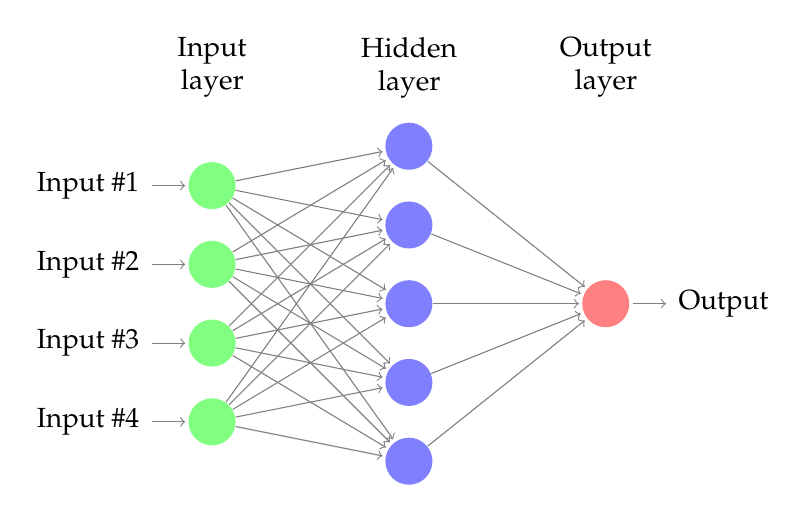
\begin{tikzpicture}[shorten >=1pt,->,draw=black!50, node distance=\layersep]
    \tikzstyle{every pin edge}=[<-,shorten <=1pt]
    \tikzstyle{neuron}=[circle,fill=black!25,minimum size=17pt,inner sep=0pt]
    \tikzstyle{input neuron}=[neuron, fill=green!50];
    \tikzstyle{output neuron}=[neuron, fill=red!50];
    \tikzstyle{hidden neuron}=[neuron, fill=blue!50];
    \tikzstyle{annot} = [text width=4em, text centered]

    % Draw the input layer nodes
    \foreach \name / \y in {1,...,4}
    % This is the same as writing \foreach \name / \y in {1/1,2/2,3/3,4/4}
        \node[input neuron, pin=left:Input \#\y] (I-\name) at (0,-\y) {};

    % Draw the hidden layer nodes
    \foreach \name / \y in {1,...,5}
        \path[yshift=0.5cm]
            node[hidden neuron] (H-\name) at (\layersep,-\y cm) {};

    % Draw the output layer node
    \node[output neuron,pin={[pin edge={->}]right:Output}, right of=H-3] (O) {};

    % Connect every node in the input layer with every node in the
    % hidden layer.
    \foreach \source in {1,...,4}
        \foreach \dest in {1,...,5}
            \path (I-\source) edge (H-\dest);

    % Connect every node in the hidden layer with the output layer
    \foreach \source in {1,...,5}
        \path (H-\source) edge (O);

    % Annotate the layers
    \node[annot,above of=H-1, node distance=1cm] (hl) {Hidden layer};
    \node[annot,left of=hl] {Input layer};
    \node[annot,right of=hl] {Output layer};
\end{tikzpicture}
%\caption{Artificial neural network}
\centering
\caption{Shallow neural networks with one hidden layer}
\end{figure}
ANN has drawn attention from well testing researchers since the 1990s. An early application in well testing was introduced by Al-Kaabi and Lee (1990) to identify the interpretation models from derivative plots. Juniardi and Ershaghi (1993) studied the complexities of using ANN with a focus on well test analysis of faulted reservoirs, and discussed some of the shortcomings of the ANN method. Around the same time, Ershaghi et al. (1993) proposed an enhanced approach based on the work of Al-Kaabi and Lee (1990), by training multiple ANNs where each neural net was designed to learn the patterns for a specific reservoir model. In 1995, Athichanagorn and Horne combined ANN with sequential predictive probability method to improve the accuracy of interpretation. ANN was used to generate initial parameter estimates of the candidate reservoir models that it identified. The candidate models and initial estimates were then passed to the sequential predictive probability method for final evaluations.

\subsubsection{Deep feed-foward networks}
Deep feedforward networks, also called feedforward neural networks, or multilayer perceptron (MLPS), are the quintessential learning models. The goal of a feedforward networks is to approximate some function f. For example, for a classifier, $y = f(x)$ maps an in put $\textbf{x}$ to a category y. A feedforward networks defines a mapping $\mathbf{y} = f(\mathbf{x},\mathbf{\theta})$ and learns the values of parameters $\mathbf{\theta}$ that the result in the best function approximation.\cite{Ian}

\begin{figure}[H]
\centering
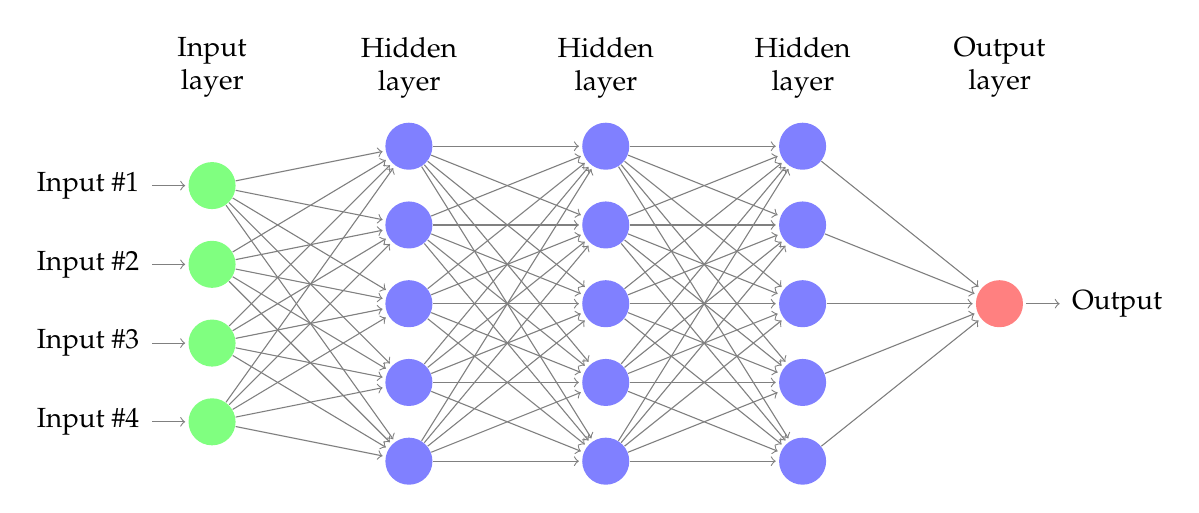
\begin{tikzpicture}[shorten >=1pt,->,draw=black!50, node distance=\layersep]
    \tikzstyle{every pin edge}=[<-,shorten <=1pt]
    \tikzstyle{neuron}=[circle,fill=black!25,minimum size=17pt,inner sep=0pt]
    \tikzstyle{input neuron}=[neuron, fill=green!50];
    \tikzstyle{output neuron}=[neuron, fill=red!50];
    \tikzstyle{hidden neuron1}=[neuron, fill=blue!50];
    \tikzstyle{hidden neuron2}=[neuron, fill=blue!50];
    \tikzstyle{hidden neuron3}=[neuron, fill=blue!50];
    \tikzstyle{annot} = [text width=4em, text centered]

    % Draw the input layer nodes
    \foreach \name / \y in {1,...,4}
    % This is the same as writing \foreach \name / \y in {1/1,2/2,3/3,4/4}
        \node[input neuron, pin=left:Input \#\y] (I-\name) at (0,-\y) {};

    % Draw the hidden layer nodes
    \foreach \name / \y in {1,...,5}
        \path[yshift=0.5cm]
            node[hidden neuron1] (H1-\name) at (\layersep,-\y cm) {};

    \foreach \name / \y in {1,...,5}
        \path[yshift=0.5cm]
            node[hidden neuron2] (H2-\name) at (\layersep +\layersep,-\y cm) {};

    \foreach \name / \y in {1,...,5}
        \path[yshift=0.5cm]
            node[hidden neuron3] (H3-\name) at (\layersep+\layersep+\layersep,-\y cm) {};
    % Draw the output layer node
    \node[output neuron,pin={[pin edge={->}]right:Output}, right of=H3-3] (O) {};

    % Connect every node in the input layer with every node in the
    % hidden layer.
    \foreach \source in {1,...,4}
        \foreach \dest in {1,...,5}
            \path (I-\source) edge (H1-\dest);
    \foreach \source in {1,...,5}
        \foreach \dest in {1,...,5}
            \path (H1-\source) edge (H2-\dest);
    \foreach \source in {1,...,5}
        \foreach \dest in {1,...,5}
            \path (H2-\source) edge (H3-\dest);
    % Connect every node in the hidden layer with the output layer
    \foreach \source in {1,...,5}
        \path (H3-\source) edge (O);

    % Annotate the layers
    \node[annot,above of=H1-1, node distance=1cm] (hl1) {Hidden layer};
    \node[annot,above of=H2-1, node distance=1cm] (hl2) {Hidden layer};
    \node[annot,above of=H3-1, node distance=1cm] (hl3) {Hidden layer};
    \node[annot,left of=hl1] {Input layer};
    \node[annot,right of=hl3] {Output layer};
\end{tikzpicture}
\caption{Deep feed forward neural networks}
\end{figure}
Recently, deep feed forward neural networks (or deep neural networks) has been applied widely in oil and gas industry. A new approach to reservoir characterization using deep neural netwokrs has been introduced by M. Korjani, Andrei Popa, Eli Grijalva, and Steve Cassidy \cite{example1}; wellbore stability prediction \cite{example2}; Deep recurrent neural network for surface pressure respone during the hydraulics fracturing process \cite{example3}; Deep neural network based prediction of Leak-Off Pressure in Offshore Norway \cite{example4}; New method for extracting the work status in Shipyard using Deep Neural Networks \cite{example5}; diagnostics of rod pumps with use of deep neural networks \cite{example7}; Automatic salt-body classification using a deep convolutional neural network \cite{example8}; seismic problems has been issued by deep neural networks in various papers such as: deep neural network architectures arising in seismic inverse problems\cite{example6}; Application of convolutional and deep neural networks for GPU based seismic interpretations \cite{example9}. Beside, deep convolutional neural networks has also been built for geology problems: Deep Learning Convolutional Neural Networks to Predict Porous Media Properties \cite{example10}, Visual explanations from convolutional neural networks for fault detection\cite{example11}.

%\subsubsection{Restricted Boltzmann Machines}
%\subsubsection{Convolutional neural networks}
%Convolutional neural networks (CNNs, or ConvNets) are essential tools for deep learning, and are especially suited for analyzing image data. For example, you can use CNNs to classify images. To predict continuous data, such as angles and distances, you can include a regression layer at the end of the network.
\subsubsection{Simple Recurrent neural networks}
Recurrent neural networks (RNNs) exploit characteristics of a feedback network, allowing the model to construct a sequential representation of input data. However, simple RNNs have been notoriously difficult to train, due to their iterative nature and the highly volatile relationship between the parameters and the hidden states \cite{Bengio}.\\
The network is given a sequence of inputs. Then, the network computes a sequence of hidden states and a sequence of predictions for each step in time. The sequences are computed by iterating through a series of equations that updates the model’s weight matrices, hidden layers, and the output units. The RNN utilizes predefined vector-valued functions that contain a computable Jacobian and are typically non-linear and applied coordinate-wise\cite{Mar}.
\begin{figure}[H]
  \centering
  \fbox{\includegraphics[scale=0.2]{Fig/RNN.png}}
  \caption{Recurrent neural network simple architechture\cite{LSTM}}
\end{figure}

\subsubsection{Long short term memory}
Long short-term memory (LSTM) units (or blocks) are a building unit for layers of a recurrent neural network (RNN). A RNN composed of LSTM units is often called an LSTM network. A common LSTM unit is composed of a cell, an input gate, an output gate and a forget gate. The cell is responsible for "remembering" values over arbitrary time intervals; hence the word "memory" in LSTM. Each of the three gates can be thought of as a "conventional" artificial neuron, as in a multi-layer (or feedforward) neural network: that is, they compute an activation (using an activation function) of a weighted sum. Intuitively, they can be thought as regulators of the flow of values that goes through the connections of the LSTM; hence the denotation gate and there are connections between these gates and the cell. A detailed explanation has been introduced by Colah in his blog about long short term memory\cite{LSTM}.
\begin{figure}[H]
    \centering
    \fbox{\includegraphics[scale=0.4]{Fig/LSTM.png}}
    \caption{Simple stretch of long short term memory\cite{LSTM}}
\end{figure}


\subsubsection{Gated Recurrent Unit}
In simple words, the GRU unit does not have to use a memory unit to control the flow of information like the LSTM unit. It can directly makes use of the all hidden states without any control. GRUs have fewer parameters and thus may train a bit faster or need less data to generalize. But, with large data, the LSTMs with higher expressiveness may lead to better results.\\
They are almost similar to LSTMs except that they have two gates: reset gate and update gate. Reset gate determines how to combine new input to previous memory and update gate determines how much of the previous state to keep. Update gate in GRU is what input gate and forget gate were in LSTM. We don't have the second non linearity in GRU before calculating the outpu, neither they have the output gate.
\begin{figure}[H]
  \centering
  \fbox{\includegraphics[scale=0.4]{Fig/GRU.png}}
  \caption{Simple stretch of Gated Recurrent Unit\cite{LSTM}}
\end{figure}




\clearpage
\section{Methodology}
\subsection{Input data}
The production dataset used in this paper is from Volve field on Norwegian continental shelf with around 8 years history. Daily oil, gas and water production data are all recorded consist with pressure, temperature and choke size as operation constraint. These production data are the main input variables for the machine learning and deep learning model, and it gives multi-phase production predictions in the future as model output.\\
Starting in February 2008, the Volve production lasted for about eight years. At peak, the field produced 56,000 barrels per day, and a total of 63 million barrels of oil were produced before the field was shut down in 2016. The field was developed when the oil price was low, and an unconventional concept was chosen to recover the resources in an easy and profitable manner. The field data will now have a new life. The Volve licensees were ExxonMobil and Bayerngas. Information about geology, geophysics, drilling, static models, dynamic simulations and other information has provied by Equinor company in 2018\cite{Volve}.\\
In this research, bottom hole pressure (BHP), tubing head pressure (THP), bottom hole temperature (BHT), well head temperature (WHT), different pressure in casing (DP), choke size (CS) in percentage is the input for training machine learning and deep learning algorithms.
\subsection{Work-flow}
\begin{figure}[H]
\centering


\tikzset{every picture/.style={line width=0.75pt}} %set default line width to 0.75pt        

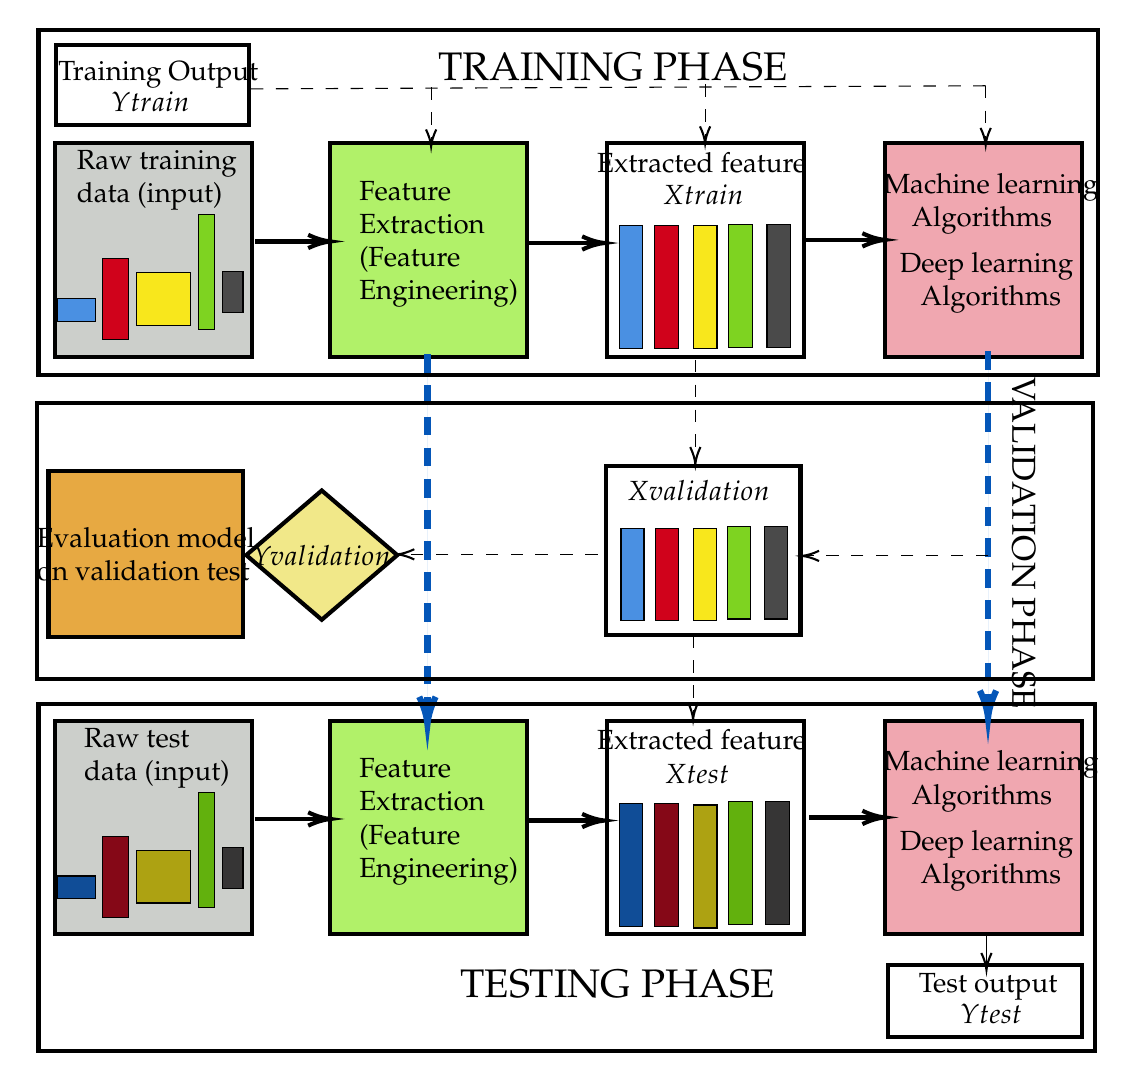
\begin{tikzpicture}[x=0.75pt,y=0.75pt,yscale=-0.75,xscale=0.75]
%uncomment if require: \path (0,991); %set diagram left start at 0, and has height of 991

%Shape: Rectangle [id:dp33352411430245066] 
\draw  [fill={rgb, 255:red, 204; green, 207; blue, 203 }  ,fill opacity=1 ][line width=1.5]  (90.5,112) -- (217.01,112) -- (217.01,249.09) -- (90.5,249.09) -- cycle ;
%Shape: Rectangle [id:dp6057047748357903] 
\draw  [fill={rgb, 255:red, 74; green, 144; blue, 226 }  ,fill opacity=1 ] (92.36,211.62) -- (116.55,211.62) -- (116.55,226.24) -- (92.36,226.24) -- cycle ;
%Shape: Rectangle [id:dp6693239668689327] 
\draw  [fill={rgb, 255:red, 74; green, 74; blue, 74 }  ,fill opacity=1 ] (198.4,194.25) -- (211.43,194.25) -- (211.43,220.75) -- (198.4,220.75) -- cycle ;
%Shape: Rectangle [id:dp5166619474253886] 
\draw  [fill={rgb, 255:red, 248; green, 231; blue, 28 }  ,fill opacity=1 ] (143.06,195.17) -- (177.47,195.17) -- (177.47,228.98) -- (143.06,228.98) -- cycle ;
%Shape: Rectangle [id:dp05336156565238592] 
\draw  [fill={rgb, 255:red, 126; green, 211; blue, 33 }  ,fill opacity=1 ] (182.59,157.7) -- (192.82,157.7) -- (192.82,231.72) -- (182.59,231.72) -- cycle ;
%Shape: Rectangle [id:dp7498108270270376] 
\draw  [fill={rgb, 255:red, 208; green, 2; blue, 27 }  ,fill opacity=1 ] (121.2,186.03) -- (137.94,186.03) -- (137.94,238.12) -- (121.2,238.12) -- cycle ;
%Shape: Rectangle [id:dp6385740702069653] 
\draw  [fill={rgb, 255:red, 177; green, 241; blue, 105 }  ,fill opacity=1 ][line width=1.5]  (267.24,112) -- (393.75,112) -- (393.75,249.09) -- (267.24,249.09) -- cycle ;
%Shape: Rectangle [id:dp817781736137955] 
\draw  [line width=1.5]  (445.07,111.91) -- (571.58,111.91) -- (571.58,249) -- (445.07,249) -- cycle ;
%Shape: Rectangle [id:dp014778479576159742] 
\draw  [fill={rgb, 255:red, 240; green, 167; blue, 176 }  ,fill opacity=1 ][line width=1.5]  (623.99,111.91) -- (750.5,111.91) -- (750.5,249) -- (623.99,249) -- cycle ;
%Shape: Rectangle [id:dp39082390906042375] 
\draw  [fill={rgb, 255:red, 74; green, 144; blue, 226 }  ,fill opacity=1 ] (453,165) -- (468.23,165) -- (468.23,244) -- (453,244) -- cycle ;
%Shape: Rectangle [id:dp6539080299135681] 
\draw  [fill={rgb, 255:red, 208; green, 2; blue, 27 }  ,fill opacity=1 ] (475.65,165) -- (490.88,165) -- (490.88,244) -- (475.65,244) -- cycle ;
%Shape: Rectangle [id:dp4947111637383488] 
\draw  [fill={rgb, 255:red, 248; green, 231; blue, 28 }  ,fill opacity=1 ] (500.65,165) -- (515.88,165) -- (515.88,244) -- (500.65,244) -- cycle ;
%Shape: Rectangle [id:dp177399350430142] 
\draw  [fill={rgb, 255:red, 126; green, 211; blue, 33 }  ,fill opacity=1 ] (523.27,164) -- (538.5,164) -- (538.5,243) -- (523.27,243) -- cycle ;
%Shape: Rectangle [id:dp3339883555880957] 
\draw  [fill={rgb, 255:red, 74; green, 74; blue, 74 }  ,fill opacity=1 ] (548,164) -- (563.23,164) -- (563.23,243) -- (548,243) -- cycle ;
%Straight Lines [id:da32669073592535447] 
\draw  [dash pattern={on 4.5pt off 4.5pt}]  (216.5,77) -- (688.5,75) ;


%Straight Lines [id:da8578618600473429] 
\draw [line width=1.5]    (219,175) -- (264.5,175) ;
\draw [shift={(267.5,175)}, rotate = 180] [color={rgb, 255:red, 0; green, 0; blue, 0 }  ][line width=1.5]    (14.21,-4.28) .. controls (9.04,-1.82) and (4.3,-0.39) .. (0,0) .. controls (4.3,0.39) and (9.04,1.82) .. (14.21,4.28)   ;

%Straight Lines [id:da8510737319968585] 
\draw [line width=1.5]    (395,176) -- (440.5,176) ;
\draw [shift={(443.5,176)}, rotate = 180] [color={rgb, 255:red, 0; green, 0; blue, 0 }  ][line width=1.5]    (14.21,-4.28) .. controls (9.04,-1.82) and (4.3,-0.39) .. (0,0) .. controls (4.3,0.39) and (9.04,1.82) .. (14.21,4.28)   ;

%Straight Lines [id:da6514923239736802] 
\draw [line width=1.5]    (571.5,174) -- (620.5,174) ;
\draw [shift={(623.5,174)}, rotate = 180] [color={rgb, 255:red, 0; green, 0; blue, 0 }  ][line width=1.5]    (14.21,-4.28) .. controls (9.04,-1.82) and (4.3,-0.39) .. (0,0) .. controls (4.3,0.39) and (9.04,1.82) .. (14.21,4.28)   ;

%Straight Lines [id:da9555017551246445] 
\draw  [dash pattern={on 4.5pt off 4.5pt}]  (332.25,76) -- (332.25,112) ;
\draw [shift={(332.25,114)}, rotate = 270] [color={rgb, 255:red, 0; green, 0; blue, 0 }  ][line width=0.75]    (10.93,-3.29) .. controls (6.95,-1.4) and (3.31,-0.3) .. (0,0) .. controls (3.31,0.3) and (6.95,1.4) .. (10.93,3.29)   ;

%Straight Lines [id:da347318891325479] 
\draw  [dash pattern={on 4.5pt off 4.5pt}]  (508.25,74) -- (508.25,110) ;
\draw [shift={(508.25,112)}, rotate = 270] [color={rgb, 255:red, 0; green, 0; blue, 0 }  ][line width=0.75]    (10.93,-3.29) .. controls (6.95,-1.4) and (3.31,-0.3) .. (0,0) .. controls (3.31,0.3) and (6.95,1.4) .. (10.93,3.29)   ;

%Straight Lines [id:da1789703386773951] 
\draw  [dash pattern={on 4.5pt off 4.5pt}]  (688.5,75) -- (688.5,111) ;
\draw [shift={(688.5,113)}, rotate = 270] [color={rgb, 255:red, 0; green, 0; blue, 0 }  ][line width=0.75]    (10.93,-3.29) .. controls (6.95,-1.4) and (3.31,-0.3) .. (0,0) .. controls (3.31,0.3) and (6.95,1.4) .. (10.93,3.29)   ;

%Shape: Rectangle [id:dp9145279844922068] 
\draw  [fill={rgb, 255:red, 204; green, 207; blue, 203 }  ,fill opacity=1 ][line width=1.5]  (90.5,483) -- (217.01,483) -- (217.01,620.09) -- (90.5,620.09) -- cycle ;
%Shape: Rectangle [id:dp6105978246834138] 
\draw  [fill={rgb, 255:red, 16; green, 77; blue, 151 }  ,fill opacity=1 ] (92.36,582.62) -- (116.55,582.62) -- (116.55,597.24) -- (92.36,597.24) -- cycle ;
%Shape: Rectangle [id:dp807654593297555] 
\draw  [fill={rgb, 255:red, 54; green, 53; blue, 53 }  ,fill opacity=1 ] (198.4,564.25) -- (211.43,564.25) -- (211.43,590.75) -- (198.4,590.75) -- cycle ;
%Shape: Rectangle [id:dp3465544458705201] 
\draw  [fill={rgb, 255:red, 173; green, 162; blue, 18 }  ,fill opacity=1 ] (143.06,566.17) -- (177.47,566.17) -- (177.47,599.98) -- (143.06,599.98) -- cycle ;
%Shape: Rectangle [id:dp4995002073003202] 
\draw  [fill={rgb, 255:red, 98; green, 177; blue, 13 }  ,fill opacity=1 ] (182.59,528.7) -- (192.82,528.7) -- (192.82,602.72) -- (182.59,602.72) -- cycle ;
%Shape: Rectangle [id:dp7549134162941816] 
\draw  [fill={rgb, 255:red, 133; green, 8; blue, 23 }  ,fill opacity=1 ] (121.2,557.03) -- (137.94,557.03) -- (137.94,609.12) -- (121.2,609.12) -- cycle ;
%Shape: Rectangle [id:dp00852933237366893] 
\draw  [fill={rgb, 255:red, 177; green, 241; blue, 105 }  ,fill opacity=1 ][line width=1.5]  (267.24,483) -- (393.75,483) -- (393.75,620.09) -- (267.24,620.09) -- cycle ;
%Shape: Rectangle [id:dp16062313288424168] 
\draw  [line width=1.5]  (445.07,482.91) -- (571.58,482.91) -- (571.58,620) -- (445.07,620) -- cycle ;
%Shape: Rectangle [id:dp7524247322931004] 
\draw  [fill={rgb, 255:red, 240; green, 167; blue, 176 }  ,fill opacity=1 ][line width=1.5]  (623.99,482.91) -- (750.5,482.91) -- (750.5,620) -- (623.99,620) -- cycle ;
%Shape: Rectangle [id:dp2846382487532757] 
\draw  [fill={rgb, 255:red, 16; green, 77; blue, 151 }  ,fill opacity=1 ] (453,536) -- (468.23,536) -- (468.23,615) -- (453,615) -- cycle ;
%Shape: Rectangle [id:dp798945131910472] 
\draw  [fill={rgb, 255:red, 133; green, 8; blue, 23 }  ,fill opacity=1 ] (475.65,536) -- (490.88,536) -- (490.88,615) -- (475.65,615) -- cycle ;
%Shape: Rectangle [id:dp3141539680496067] 
\draw  [fill={rgb, 255:red, 173; green, 162; blue, 18 }  ,fill opacity=1 ] (500.65,537) -- (515.88,537) -- (515.88,616) -- (500.65,616) -- cycle ;
%Shape: Rectangle [id:dp10691049560331767] 
\draw  [fill={rgb, 255:red, 98; green, 177; blue, 13 }  ,fill opacity=1 ] (523.27,535) -- (538.5,535) -- (538.5,614) -- (523.27,614) -- cycle ;
%Shape: Rectangle [id:dp3066549577326315] 
\draw  [fill={rgb, 255:red, 54; green, 53; blue, 53 }  ,fill opacity=1 ] (547,535) -- (562.23,535) -- (562.23,614) -- (547,614) -- cycle ;
%Straight Lines [id:da3561377076904969] 
\draw [line width=1.5]    (219,546) -- (264.5,546) ;
\draw [shift={(267.5,546)}, rotate = 180] [color={rgb, 255:red, 0; green, 0; blue, 0 }  ][line width=1.5]    (14.21,-4.28) .. controls (9.04,-1.82) and (4.3,-0.39) .. (0,0) .. controls (4.3,0.39) and (9.04,1.82) .. (14.21,4.28)   ;

%Straight Lines [id:da34722090949242546] 
\draw [line width=1.5]    (395,547) -- (440.5,547) ;
\draw [shift={(443.5,547)}, rotate = 180] [color={rgb, 255:red, 0; green, 0; blue, 0 }  ][line width=1.5]    (14.21,-4.28) .. controls (9.04,-1.82) and (4.3,-0.39) .. (0,0) .. controls (4.3,0.39) and (9.04,1.82) .. (14.21,4.28)   ;

%Straight Lines [id:da6461688450148553] 
\draw [line width=1.5]    (575,545) -- (620.5,545) ;
\draw [shift={(623.5,545)}, rotate = 180] [color={rgb, 255:red, 0; green, 0; blue, 0 }  ][line width=1.5]    (14.21,-4.28) .. controls (9.04,-1.82) and (4.3,-0.39) .. (0,0) .. controls (4.3,0.39) and (9.04,1.82) .. (14.21,4.28)   ;

%Shape: Rectangle [id:dp11741617104471569] 
\draw  [line width=1.5]  (91.5,100) -- (215.5,100) -- (215.5,49) -- (91.5,49) -- cycle ;
%Shape: Rectangle [id:dp08540982740970204] 
\draw  [line width=1.5]  (444.5,319.39) -- (569.5,319.39) -- (569.5,428) -- (444.5,428) -- cycle ;
%Shape: Rectangle [id:dp6465075851924112] 
\draw  [fill={rgb, 255:red, 74; green, 144; blue, 226 }  ,fill opacity=1 ] (454.21,359.13) -- (469.02,359.13) -- (469.02,418.26) -- (454.21,418.26) -- cycle ;
%Shape: Rectangle [id:dp9987718602015557] 
\draw  [fill={rgb, 255:red, 208; green, 2; blue, 27 }  ,fill opacity=1 ] (476.24,359.13) -- (491.05,359.13) -- (491.05,418.26) -- (476.24,418.26) -- cycle ;
%Shape: Rectangle [id:dp5655356428056167] 
\draw  [fill={rgb, 255:red, 248; green, 231; blue, 28 }  ,fill opacity=1 ] (500.54,359.13) -- (515.35,359.13) -- (515.35,418.26) -- (500.54,418.26) -- cycle ;
%Shape: Rectangle [id:dp4389439560545667] 
\draw  [fill={rgb, 255:red, 126; green, 211; blue, 33 }  ,fill opacity=1 ] (522.53,358.38) -- (537.34,358.38) -- (537.34,417.51) -- (522.53,417.51) -- cycle ;
%Shape: Rectangle [id:dp5616078444948048] 
\draw  [fill={rgb, 255:red, 74; green, 74; blue, 74 }  ,fill opacity=1 ] (546.58,358.38) -- (561.39,358.38) -- (561.39,417.51) -- (546.58,417.51) -- cycle ;
%Straight Lines [id:da12840945198866716] 
\draw  [dash pattern={on 4.5pt off 4.5pt}]  (501.98,251) -- (501.98,316) ;
\draw [shift={(501.98,318)}, rotate = 270] [color={rgb, 255:red, 0; green, 0; blue, 0 }  ][line width=0.75]    (10.93,-3.29) .. controls (6.95,-1.4) and (3.31,-0.3) .. (0,0) .. controls (3.31,0.3) and (6.95,1.4) .. (10.93,3.29)   ;

%Shape: Rectangle [id:dp3975478474138766] 
\draw  [fill={rgb, 255:red, 231; green, 169; blue, 66 }  ,fill opacity=1 ][line width=1.5]  (86.5,322.39) -- (211.5,322.39) -- (211.5,429) -- (86.5,429) -- cycle ;
%Straight Lines [id:da5069860880844238] 
\draw  [dash pattern={on 4.5pt off 4.5pt}]  (439.25,376) -- (312.5,376) ;
\draw [shift={(310.5,376)}, rotate = 360] [color={rgb, 255:red, 0; green, 0; blue, 0 }  ][line width=0.75]    (10.93,-3.29) .. controls (6.95,-1.4) and (3.31,-0.3) .. (0,0) .. controls (3.31,0.3) and (6.95,1.4) .. (10.93,3.29)   ;

%Straight Lines [id:da4272333491970457] 
\draw [color={rgb, 255:red, 4; green, 86; blue, 184 }  ,draw opacity=1 ][fill={rgb, 255:red, 74; green, 144; blue, 226 }  ,fill opacity=1 ][line width=2.25]  [dash pattern={on 6.75pt off 4.5pt}]  (690,245.5) -- (690,477) ;
\draw [shift={(690,481)}, rotate = 270] [color={rgb, 255:red, 4; green, 86; blue, 184 }  ,draw opacity=1 ][line width=2.25]    (17.49,-5.26) .. controls (11.12,-2.23) and (5.29,-0.48) .. (0,0) .. controls (5.29,0.48) and (11.12,2.23) .. (17.49,5.26)   ;

%Straight Lines [id:da23842498234195153] 
\draw [color={rgb, 255:red, 4; green, 86; blue, 184 }  ,draw opacity=1 ][fill={rgb, 255:red, 74; green, 144; blue, 226 }  ,fill opacity=1 ][line width=2.25]  [dash pattern={on 6.75pt off 4.5pt}]  (329.88,247.5) -- (329.88,481) ;
\draw [shift={(329.88,485)}, rotate = 270] [color={rgb, 255:red, 4; green, 86; blue, 184 }  ,draw opacity=1 ][line width=2.25]    (17.49,-5.26) .. controls (11.12,-2.23) and (5.29,-0.48) .. (0,0) .. controls (5.29,0.48) and (11.12,2.23) .. (17.49,5.26)   ;

%Straight Lines [id:da46297394773208955] 
\draw  [dash pattern={on 4.5pt off 4.5pt}]  (500.54,428) -- (500.54,480) ;
\draw [shift={(500.54,482)}, rotate = 270] [color={rgb, 255:red, 0; green, 0; blue, 0 }  ][line width=0.75]    (10.93,-3.29) .. controls (6.95,-1.4) and (3.31,-0.3) .. (0,0) .. controls (3.31,0.3) and (6.95,1.4) .. (10.93,3.29)   ;

%Straight Lines [id:da13242273231572632] 
\draw  [dash pattern={on 4.5pt off 4.5pt}]  (690,377) -- (572.5,377) ;
\draw [shift={(570.5,377)}, rotate = 360] [color={rgb, 255:red, 0; green, 0; blue, 0 }  ][line width=0.75]    (10.93,-3.29) .. controls (6.95,-1.4) and (3.31,-0.3) .. (0,0) .. controls (3.31,0.3) and (6.95,1.4) .. (10.93,3.29)   ;

%Shape: Rectangle [id:dp5277043429916338] 
\draw  [line width=1.5]  (625.5,640) -- (750.5,640) -- (750.5,686) -- (625.5,686) -- cycle ;
%Straight Lines [id:da00015408678780248763] 
\draw    (689,621) -- (689,641) ;
\draw [shift={(689,643)}, rotate = 270] [color={rgb, 255:red, 0; green, 0; blue, 0 }  ][line width=0.75]    (10.93,-3.29) .. controls (6.95,-1.4) and (3.31,-0.3) .. (0,0) .. controls (3.31,0.3) and (6.95,1.4) .. (10.93,3.29)   ;

%Shape: Rectangle [id:dp4580915433425652] 
\draw  [color={rgb, 255:red, 0; green, 0; blue, 0 }  ,draw opacity=1 ][line width=1.5]  (80,39) -- (760.5,39) -- (760.5,261) -- (80,261) -- cycle ;
%Shape: Rectangle [id:dp07788141789894654] 
\draw  [line width=1.5]  (79,279) -- (757.5,279) -- (757.5,456) -- (79,456) -- cycle ;
%Shape: Rectangle [id:dp40183222780271843] 
\draw  [line width=1.5]  (80,472) -- (758.5,472) -- (758.5,695) -- (80,695) -- cycle ;
%Shape: Diamond [id:dp6980358188977897] 
\draw  [fill={rgb, 255:red, 241; green, 232; blue, 137 }  ,fill opacity=1 ][line width=1.5]  (262,335) -- (310.5,376.5) -- (262,418) -- (213.5,376.5) -- cycle ;

% Text Node
\draw (156.08,135.76) node  [align=left] {Raw training\\data (input)};
% Text Node
\draw (337.08,176.76) node  [align=left] {Feature \\Extraction\\(Feature\\Engineering)};
% Text Node
\draw (506.08,134.76) node  [align=left] {Extracted feature\\};
% Text Node
\draw (692.08,150.76) node  [align=left] {Machine learning\\ \ \ \ \ Algorithms};
% Text Node
\draw (689.08,201.76) node  [align=left] {Deep learning\\ \ \ \ Algorithms};
% Text Node
\draw (156.08,506.76) node  [align=left] {Raw test\\data (input)};
% Text Node
\draw (337.08,547.76) node  [align=left] {Feature \\Extraction\\(Feature\\Engineering)};
% Text Node
\draw (506.08,505.76) node  [align=left] {Extracted feature\\};
% Text Node
\draw (692.08,521.76) node  [align=left] {Machine learning\\ \ \ \ \ Algorithms};
% Text Node
\draw (689.08,572.76) node  [align=left] {Deep learning\\ \ \ \ Algorithms};
% Text Node
\draw (157,68) node  [align=left] {Training Output};
% Text Node
\draw (149,375.7) node  [align=left] {Evaluation model\\on validation test};
% Text Node
\draw (690,654) node  [align=left] {Test output};
% Text Node
\draw (452,652) node [scale=1.44] [align=left] {TESTING PHASE};
% Text Node
\draw (449,63) node [scale=1.44] [align=left] {TRAINING PHASE};
% Text Node
\draw (713,369) node [scale=1.2,rotate=-90] [align=left] {VALIDATION PHASE};
% Text Node
\draw (262,376.5) node   {$Yvalidation$};
% Text Node
\draw (692,671) node   {$Ytest$};
% Text Node
\draw (152,85) node   {$Ytrain$};
% Text Node
\draw (503,517) node   {$Xtest$};
% Text Node
\draw (504,335) node   {$Xvalidation$};
% Text Node
\draw (507,145) node   {$Xtrain$};


\end{tikzpicture}

\caption{Work flow for using machine and deep learning algorithms}
\end{figure}

Almost every machine learning and deep learning algorithm has followed this work-flow above. Firslt, all raw data need to be collected altogether. Feature engineering means he process of using domain knowledge of the data to create features that make machine learning algorithms work. Feature engineering is an informal topic, but it is considered essential in applied machine learning\cite{feature}. From Andrew Ng, a famous Professor in AI :"Applied machine learning is basically feature engineering".


\begin{figure}[H]
\centering


\tikzset{every picture/.style={line width=0.75pt}} %set default line width to 0.75pt        

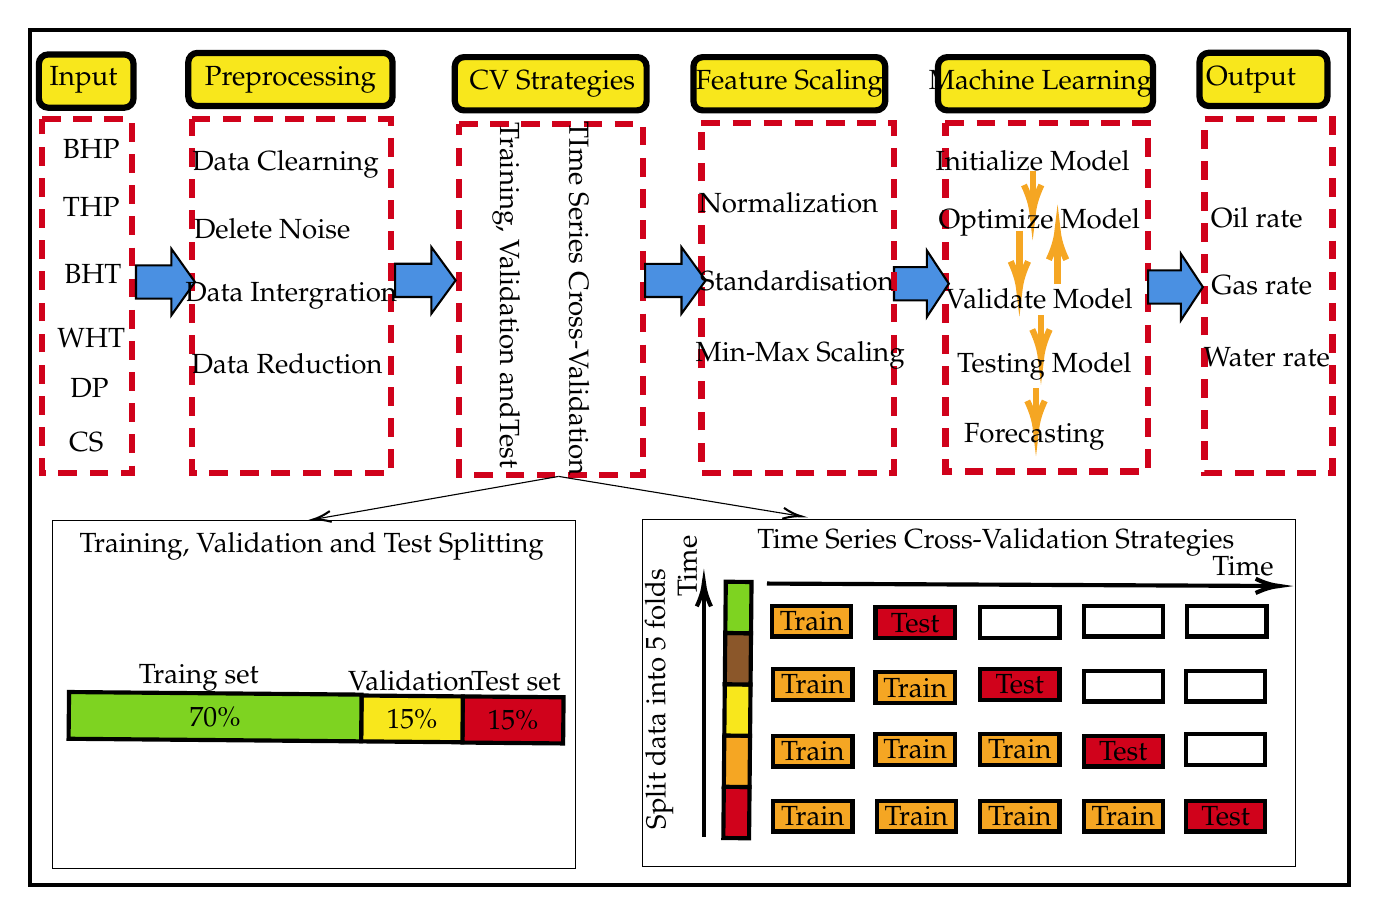
\begin{tikzpicture}[x=0.75pt,y=0.75pt,yscale=-0.8,xscale=0.8]
%uncomment if require: \path (0,805); %set diagram left start at 0, and has height of 805

%Shape: Rectangle [id:dp07853822546541556] 
\draw  [color={rgb, 255:red, 208; green, 2; blue, 27 }  ,draw opacity=1 ][dash pattern={on 6.75pt off 4.5pt}][line width=2.25]  (16.5,77.94) -- (70.5,77.94) -- (70.5,291) -- (16.5,291) -- cycle ;
%Shape: Rectangle [id:dp3676508384424104] 
\draw  [color={rgb, 255:red, 208; green, 2; blue, 27 }  ,draw opacity=1 ][dash pattern={on 6.75pt off 4.5pt}][line width=2.25]  (106.5,77.94) -- (226.5,77.94) -- (226.5,291) -- (106.5,291) -- cycle ;
%Shape: Rectangle [id:dp17843254528937924] 
\draw  [color={rgb, 255:red, 208; green, 2; blue, 27 }  ,draw opacity=1 ][dash pattern={on 6.75pt off 4.5pt}][line width=2.25]  (267.5,80.94) -- (378.5,80.94) -- (378.5,292) -- (267.5,292) -- cycle ;
%Shape: Rectangle [id:dp7714269448540817] 
\draw  [color={rgb, 255:red, 208; green, 2; blue, 27 }  ,draw opacity=1 ][dash pattern={on 6.75pt off 4.5pt}][line width=2.25]  (560.5,79.94) -- (682.5,79.94) -- (682.5,290) -- (560.5,290) -- cycle ;
%Right Arrow [id:dp4267474130020711] 
\draw  [fill={rgb, 255:red, 74; green, 144; blue, 226 }  ,fill opacity=1 ][line width=0.75]  (73,165.94) -- (94.3,165.94) -- (94.3,155.94) -- (108.5,175.94) -- (94.3,195.94) -- (94.3,185.94) -- (73,185.94) -- cycle ;
%Flowchart: Alternative Process [id:dp4199707331903012] 
\draw  [fill={rgb, 255:red, 248; green, 231; blue, 28 }  ,fill opacity=1 ][line width=2.25]  (556,46.1) .. controls (556,43) and (558.51,40.49) .. (561.61,40.49) -- (679.89,40.49) .. controls (682.99,40.49) and (685.5,43) .. (685.5,46.1) -- (685.5,66.94) .. controls (685.5,70.04) and (682.99,72.55) .. (679.89,72.55) -- (561.61,72.55) .. controls (558.51,72.55) and (556,70.04) .. (556,66.94) -- cycle ;
%Flowchart: Alternative Process [id:dp9589116956685553] 
\draw  [fill={rgb, 255:red, 248; green, 231; blue, 28 }  ,fill opacity=1 ][line width=2.25]  (104.5,43.54) .. controls (104.5,40.44) and (107.01,37.94) .. (110.1,37.94) -- (221.9,37.94) .. controls (224.99,37.94) and (227.5,40.44) .. (227.5,43.54) -- (227.5,64.34) .. controls (227.5,67.43) and (224.99,69.94) .. (221.9,69.94) -- (110.1,69.94) .. controls (107.01,69.94) and (104.5,67.43) .. (104.5,64.34) -- cycle ;
%Flowchart: Alternative Process [id:dp145095190178265] 
\draw  [fill={rgb, 255:red, 248; green, 231; blue, 28 }  ,fill opacity=1 ][line width=2.25]  (265,46.1) .. controls (265,43) and (267.51,40.49) .. (270.61,40.49) -- (374.89,40.49) .. controls (377.99,40.49) and (380.5,43) .. (380.5,46.1) -- (380.5,66.94) .. controls (380.5,70.04) and (377.99,72.55) .. (374.89,72.55) -- (270.61,72.55) .. controls (267.51,72.55) and (265,70.04) .. (265,66.94) -- cycle ;
%Flowchart: Alternative Process [id:dp5478801307658322] 
\draw  [color={rgb, 255:red, 0; green, 0; blue, 0 }  ,draw opacity=1 ][fill={rgb, 255:red, 248; green, 231; blue, 28 }  ,fill opacity=1 ][line width=2.25]  (14.5,44.49) .. controls (14.5,41.39) and (17.01,38.88) .. (20.11,38.88) -- (65.89,38.88) .. controls (68.99,38.88) and (71.5,41.39) .. (71.5,44.49) -- (71.5,65.33) .. controls (71.5,68.43) and (68.99,70.94) .. (65.89,70.94) -- (20.11,70.94) .. controls (17.01,70.94) and (14.5,68.43) .. (14.5,65.33) -- cycle ;
%Right Arrow [id:dp07666063439783866] 
\draw  [fill={rgb, 255:red, 74; green, 144; blue, 226 }  ,fill opacity=1 ][line width=0.75]  (229,164.94) -- (250.9,164.94) -- (250.9,154.94) -- (265.5,174.94) -- (250.9,194.94) -- (250.9,184.94) -- (229,184.94) -- cycle ;
%Right Arrow [id:dp483153462033711] 
\draw  [fill={rgb, 255:red, 74; green, 144; blue, 226 }  ,fill opacity=1 ][line width=0.75]  (529.5,166.94) -- (549.3,166.94) -- (549.3,156.94) -- (562.5,176.94) -- (549.3,196.94) -- (549.3,186.94) -- (529.5,186.94) -- cycle ;
%Straight Lines [id:da9625748638646549] 
\draw [color={rgb, 255:red, 245; green, 166; blue, 35 }  ,draw opacity=1 ][fill={rgb, 255:red, 80; green, 227; blue, 194 }  ,fill opacity=1 ][line width=2.25]    (613,109) -- (613,131) ;
\draw [shift={(613,135)}, rotate = 270] [color={rgb, 255:red, 245; green, 166; blue, 35 }  ,draw opacity=1 ][line width=2.25]    (17.49,-5.26) .. controls (11.12,-2.23) and (5.29,-0.48) .. (0,0) .. controls (5.29,0.48) and (11.12,2.23) .. (17.49,5.26)   ;

%Straight Lines [id:da09562711482553621] 
\draw [color={rgb, 255:red, 245; green, 166; blue, 35 }  ,draw opacity=1 ][line width=2.25]    (605,144.94) -- (605,177) ;
\draw [shift={(605,181)}, rotate = 270] [color={rgb, 255:red, 245; green, 166; blue, 35 }  ,draw opacity=1 ][line width=2.25]    (17.49,-5.26) .. controls (11.12,-2.23) and (5.29,-0.48) .. (0,0) .. controls (5.29,0.48) and (11.12,2.23) .. (17.49,5.26)   ;

%Straight Lines [id:da9581412762029833] 
\draw [color={rgb, 255:red, 245; green, 166; blue, 35 }  ,draw opacity=1 ][line width=2.25]    (618,195.94) -- (618,218) ;
\draw [shift={(618,222)}, rotate = 270] [color={rgb, 255:red, 245; green, 166; blue, 35 }  ,draw opacity=1 ][line width=2.25]    (17.49,-5.26) .. controls (11.12,-2.23) and (5.29,-0.48) .. (0,0) .. controls (5.29,0.48) and (11.12,2.23) .. (17.49,5.26)   ;

%Straight Lines [id:da24256442466359818] 
\draw [color={rgb, 255:red, 245; green, 166; blue, 35 }  ,draw opacity=1 ][line width=2.25]    (615,239.94) -- (615,261) ;
\draw [shift={(615,265)}, rotate = 270] [color={rgb, 255:red, 245; green, 166; blue, 35 }  ,draw opacity=1 ][line width=2.25]    (17.49,-5.26) .. controls (11.12,-2.23) and (5.29,-0.48) .. (0,0) .. controls (5.29,0.48) and (11.12,2.23) .. (17.49,5.26)   ;

%Straight Lines [id:da4633066781015024] 
\draw [color={rgb, 255:red, 245; green, 166; blue, 35 }  ,draw opacity=1 ][line width=2.25]    (628,177) -- (628,149) ;
\draw [shift={(628,145)}, rotate = 450] [color={rgb, 255:red, 245; green, 166; blue, 35 }  ,draw opacity=1 ][line width=2.25]    (17.49,-5.26) .. controls (11.12,-2.23) and (5.29,-0.48) .. (0,0) .. controls (5.29,0.48) and (11.12,2.23) .. (17.49,5.26)   ;

%Flowchart: Alternative Process [id:dp34656315790461034] 
\draw  [color={rgb, 255:red, 0; green, 0; blue, 0 }  ,draw opacity=1 ][fill={rgb, 255:red, 248; green, 231; blue, 28 }  ,fill opacity=1 ][line width=2.25]  (713.5,43.49) .. controls (713.5,40.39) and (716.01,37.88) .. (719.11,37.88) -- (784.89,37.88) .. controls (787.99,37.88) and (790.5,40.39) .. (790.5,43.49) -- (790.5,64.33) .. controls (790.5,67.43) and (787.99,69.94) .. (784.89,69.94) -- (719.11,69.94) .. controls (716.01,69.94) and (713.5,67.43) .. (713.5,64.33) -- cycle ;
%Shape: Rectangle [id:dp5583073306986339] 
\draw  [color={rgb, 255:red, 208; green, 2; blue, 27 }  ,draw opacity=1 ][dash pattern={on 6.75pt off 4.5pt}][line width=2.25]  (716.5,77.94) -- (793.5,77.94) -- (793.5,291) -- (716.5,291) -- cycle ;
%Right Arrow [id:dp8247837204105005] 
\draw  [fill={rgb, 255:red, 74; green, 144; blue, 226 }  ,fill opacity=1 ][line width=0.75]  (682.5,168.94) -- (702.3,168.94) -- (702.3,158.94) -- (715.5,178.94) -- (702.3,198.94) -- (702.3,188.94) -- (682.5,188.94) -- cycle ;
%Flowchart: Alternative Process [id:dp2567889521485418] 
\draw  [fill={rgb, 255:red, 248; green, 231; blue, 28 }  ,fill opacity=1 ][line width=2.25]  (408.72,46.1) .. controls (408.72,43) and (411.23,40.49) .. (414.33,40.49) -- (518.61,40.49) .. controls (521.71,40.49) and (524.22,43) .. (524.22,46.1) -- (524.22,66.94) .. controls (524.22,70.04) and (521.71,72.55) .. (518.61,72.55) -- (414.33,72.55) .. controls (411.23,72.55) and (408.72,70.04) .. (408.72,66.94) -- cycle ;
%Shape: Rectangle [id:dp6171734568210094] 
\draw  [color={rgb, 255:red, 208; green, 2; blue, 27 }  ,draw opacity=1 ][dash pattern={on 6.75pt off 4.5pt}][line width=2.25]  (413.5,79.94) -- (529.5,79.94) -- (529.5,291) -- (413.5,291) -- cycle ;
%Right Arrow [id:dp9280333171304811] 
\draw  [fill={rgb, 255:red, 74; green, 144; blue, 226 }  ,fill opacity=1 ][line width=0.75]  (379.6,164.97) -- (401.5,164.97) -- (401.5,154.97) -- (416.1,174.97) -- (401.5,194.97) -- (401.5,184.97) -- (379.6,184.97) -- cycle ;
%Shape: Rectangle [id:dp5304042976802675] 
\draw  [fill={rgb, 255:red, 208; green, 2; blue, 27 }  ,fill opacity=1 ][line width=1.5]  (426.7,510.78) -- (427,479.91) -- (442.5,480.06) -- (442.2,510.93) -- cycle ;
%Shape: Rectangle [id:dp389524301164212] 
\draw  [fill={rgb, 255:red, 245; green, 166; blue, 35 }  ,fill opacity=1 ][line width=1.5]  (427,479.91) -- (427.3,449.04) -- (442.8,449.19) -- (442.5,480.06) -- cycle ;
%Shape: Rectangle [id:dp06717136948438174] 
\draw  [fill={rgb, 255:red, 248; green, 231; blue, 28 }  ,fill opacity=1 ][line width=1.5]  (427.3,449.04) -- (427.59,418.17) -- (443.09,418.32) -- (442.8,449.19) -- cycle ;
%Shape: Rectangle [id:dp4741721034372983] 
\draw  [fill={rgb, 255:red, 139; green, 87; blue, 42 }  ,fill opacity=1 ][line width=1.5]  (427.59,418.17) -- (427.89,387.3) -- (443.39,387.45) -- (443.09,418.32) -- cycle ;
%Shape: Rectangle [id:dp4252187852170447] 
\draw  [fill={rgb, 255:red, 126; green, 211; blue, 33 }  ,fill opacity=1 ][line width=1.5]  (427.89,387.3) -- (428.19,356.43) -- (443.69,356.58) -- (443.39,387.45) -- cycle ;
%Straight Lines [id:da8301330510597829] 
\draw [line width=1.5]    (415,510) -- (415,360.06) ;
\draw [shift={(415,357.06)}, rotate = 450] [color={rgb, 255:red, 0; green, 0; blue, 0 }  ][line width=1.5]    (14.21,-4.28) .. controls (9.04,-1.82) and (4.3,-0.39) .. (0,0) .. controls (4.3,0.39) and (9.04,1.82) .. (14.21,4.28)   ;

%Shape: Rectangle [id:dp6398920356953457] 
\draw  [color={rgb, 255:red, 0; green, 0; blue, 0 }  ,draw opacity=1 ][fill={rgb, 255:red, 245; green, 166; blue, 35 }  ,fill opacity=1 ][line width=1.5]  (456,370.82) -- (503.83,370.82) -- (503.83,389.41) -- (456,389.41) -- cycle ;
%Shape: Rectangle [id:dp6002468814991093] 
\draw  [fill={rgb, 255:red, 208; green, 2; blue, 27 }  ,fill opacity=1 ][line width=1.5]  (518.32,371.8) -- (566.15,371.8) -- (566.15,390.39) -- (518.32,390.39) -- cycle ;
%Shape: Rectangle [id:dp4063250857893066] 
\draw  [line width=1.5]  (581.33,371.8) -- (629.16,371.8) -- (629.16,390.39) -- (581.33,390.39) -- cycle ;
%Shape: Rectangle [id:dp6339821012870924] 
\draw  [line width=1.5]  (643.66,370.82) -- (691.48,370.82) -- (691.48,389.41) -- (643.66,389.41) -- cycle ;
%Shape: Rectangle [id:dp594138053802681] 
\draw  [line width=1.5]  (705.98,370.82) -- (753.81,370.82) -- (753.81,389.41) -- (705.98,389.41) -- cycle ;
%Shape: Rectangle [id:dp05919193690656721] 
\draw  [fill={rgb, 255:red, 245; green, 166; blue, 35 }  ,fill opacity=1 ][line width=1.5]  (456.69,408.98) -- (504.52,408.98) -- (504.52,427.58) -- (456.69,427.58) -- cycle ;
%Shape: Rectangle [id:dp8218788470250212] 
\draw  [fill={rgb, 255:red, 245; green, 166; blue, 35 }  ,fill opacity=1 ][line width=1.5]  (518.32,410.94) -- (566.15,410.94) -- (566.15,429.53) -- (518.32,429.53) -- cycle ;
%Shape: Rectangle [id:dp5319802316530327] 
\draw  [fill={rgb, 255:red, 208; green, 2; blue, 27 }  ,fill opacity=1 ][line width=1.5]  (581.33,408.98) -- (629.16,408.98) -- (629.16,427.58) -- (581.33,427.58) -- cycle ;
%Shape: Rectangle [id:dp5421660810294261] 
\draw  [line width=1.5]  (643.66,409.96) -- (691.48,409.96) -- (691.48,428.56) -- (643.66,428.56) -- cycle ;
%Shape: Rectangle [id:dp7307421679592645] 
\draw  [line width=1.5]  (705.29,409.96) -- (753.11,409.96) -- (753.11,428.56) -- (705.29,428.56) -- cycle ;
%Shape: Rectangle [id:dp453421269370753] 
\draw  [fill={rgb, 255:red, 245; green, 166; blue, 35 }  ,fill opacity=1 ][line width=1.5]  (456.69,449.11) -- (504.52,449.11) -- (504.52,467.7) -- (456.69,467.7) -- cycle ;
%Shape: Rectangle [id:dp6116779059785222] 
\draw  [fill={rgb, 255:red, 245; green, 166; blue, 35 }  ,fill opacity=1 ][line width=1.5]  (518.32,448.13) -- (566.15,448.13) -- (566.15,466.72) -- (518.32,466.72) -- cycle ;
%Shape: Rectangle [id:dp4864900882623333] 
\draw  [fill={rgb, 255:red, 245; green, 166; blue, 35 }  ,fill opacity=1 ][line width=1.5]  (581.33,448.13) -- (629.16,448.13) -- (629.16,466.72) -- (581.33,466.72) -- cycle ;
%Shape: Rectangle [id:dp08243721834182594] 
\draw  [fill={rgb, 255:red, 245; green, 166; blue, 35 }  ,fill opacity=1 ][line width=1.5]  (456.69,488.25) -- (504.52,488.25) -- (504.52,506.84) -- (456.69,506.84) -- cycle ;
%Shape: Rectangle [id:dp895843857971842] 
\draw  [fill={rgb, 255:red, 245; green, 166; blue, 35 }  ,fill opacity=1 ][line width=1.5]  (519.01,488.25) -- (566.84,488.25) -- (566.84,506.84) -- (519.01,506.84) -- cycle ;
%Shape: Rectangle [id:dp32630041508148877] 
\draw  [fill={rgb, 255:red, 245; green, 166; blue, 35 }  ,fill opacity=1 ][line width=1.5]  (581.33,488.25) -- (629.16,488.25) -- (629.16,506.84) -- (581.33,506.84) -- cycle ;
%Shape: Rectangle [id:dp2640693612020737] 
\draw  [fill={rgb, 255:red, 208; green, 2; blue, 27 }  ,fill opacity=1 ][line width=1.5]  (643.66,449.11) -- (691.48,449.11) -- (691.48,467.7) -- (643.66,467.7) -- cycle ;
%Shape: Rectangle [id:dp73200941348248] 
\draw  [line width=1.5]  (705.29,448.13) -- (753.11,448.13) -- (753.11,466.72) -- (705.29,466.72) -- cycle ;
%Shape: Rectangle [id:dp32727934506027245] 
\draw  [fill={rgb, 255:red, 245; green, 166; blue, 35 }  ,fill opacity=1 ][line width=1.5]  (643.66,488.25) -- (691.48,488.25) -- (691.48,506.84) -- (643.66,506.84) -- cycle ;
%Shape: Rectangle [id:dp5893268398093748] 
\draw  [fill={rgb, 255:red, 208; green, 2; blue, 27 }  ,fill opacity=1 ][line width=1.5]  (705.29,488.25) -- (753.11,488.25) -- (753.11,506.84) -- (705.29,506.84) -- cycle ;
%Straight Lines [id:da2778869237133579] 
\draw [line width=1.5]    (453,357.53) -- (758.5,358.99) ;
\draw [shift={(761.5,359)}, rotate = 180.27] [color={rgb, 255:red, 0; green, 0; blue, 0 }  ][line width=1.5]    (14.21,-4.28) .. controls (9.04,-1.82) and (4.3,-0.39) .. (0,0) .. controls (4.3,0.39) and (9.04,1.82) .. (14.21,4.28)   ;

%Shape: Rectangle [id:dp8516430580228828] 
\draw  [line width=1.5]  (9,24) -- (803.5,24) -- (803.5,539) -- (9,539) -- cycle ;
%Shape: Rectangle [id:dp3639188282518515] 
\draw  [fill={rgb, 255:red, 208; green, 2; blue, 27 }  ,fill opacity=1 ][line width=1.5]  (269.54,453.28) -- (269.82,425.49) -- (330.5,426.03) -- (330.21,453.82) -- cycle ;
%Shape: Rectangle [id:dp8967132503739018] 
\draw  [fill={rgb, 255:red, 248; green, 231; blue, 28 }  ,fill opacity=1 ][line width=1.5]  (208.56,452.57) -- (208.85,424.95) -- (269.82,425.49) -- (269.54,453.11) -- cycle ;
%Shape: Rectangle [id:dp8758356685011385] 
\draw  [fill={rgb, 255:red, 126; green, 211; blue, 33 }  ,fill opacity=1 ][line width=1.5]  (32.38,451) -- (32.67,422.85) -- (208.85,424.42) -- (208.56,452.57) -- cycle ;
%Shape: Rectangle [id:dp8159025880270944] 
\draw   (377.98,318.7) -- (771.5,318.7) -- (771.5,528) -- (377.98,528) -- cycle ;
%Shape: Rectangle [id:dp3705954356976263] 
\draw   (22.5,319.7) -- (337.5,319.7) -- (337.5,529) -- (22.5,529) -- cycle ;
%Straight Lines [id:da7762832126826611] 
\draw    (327.5,293) -- (181.47,318.65) ;
\draw [shift={(179.5,319)}, rotate = 350.03999999999996] [color={rgb, 255:red, 0; green, 0; blue, 0 }  ][line width=0.75]    (10.93,-3.29) .. controls (6.95,-1.4) and (3.31,-0.3) .. (0,0) .. controls (3.31,0.3) and (6.95,1.4) .. (10.93,3.29)   ;

%Straight Lines [id:da8588456857745094] 
\draw    (327.5,293) -- (471.53,316.68) ;
\draw [shift={(473.5,317)}, rotate = 189.33] [color={rgb, 255:red, 0; green, 0; blue, 0 }  ][line width=0.75]    (10.93,-3.29) .. controls (6.95,-1.4) and (3.31,-0.3) .. (0,0) .. controls (3.31,0.3) and (6.95,1.4) .. (10.93,3.29)   ;


% Text Node
\draw (43.44,53.91) node  [align=left] { Input };
% Text Node
\draw (46,95.94) node  [align=left] {BHP};
% Text Node
\draw (46,130.94) node  [align=left] {THP};
% Text Node
\draw (47,170.94) node  [align=left] {BHT};
% Text Node
\draw (46,209.47) node  [align=left] {WHT};
% Text Node
\draw (43,271.94) node  [align=left] {CS};
% Text Node
\draw (45,239.94) node  [align=left] {DP};
% Text Node
\draw (166.05,53.94) node  [align=left] {Preprocessing};
% Text Node
\draw (163,104.94) node  [align=left] {Data Clearning};
% Text Node
\draw (166.5,184.47) node  [align=left] {Data Intergration};
% Text Node
\draw (164,224.94) node  [align=left] {Data Reduction};
% Text Node
\draw (466.47,56.52) node  [align=left] {Feature Scaling};
% Text Node
\draw (155,143.94) node  [align=left] {Delete Noise};
% Text Node
\draw (323.75,56.52) node  [align=left] {CV Strategies};
% Text Node
\draw (617.75,56.52) node  [align=left] {Machine Learning};
% Text Node
\draw (613,102.94) node  [align=left] {Initialize Model};
% Text Node
\draw (617,139.94) node  [align=left] {Optimize Model};
% Text Node
\draw (617,185.97) node  [align=left] {Validate Model};
% Text Node
\draw (620,226.94) node  [align=left] {Testing Model};
% Text Node
\draw (614,268.94) node  [align=left] {Forecasting};
% Text Node
\draw (744.5,53.91) node  [align=left] {Output};
% Text Node
\draw (748,136.94) node  [align=left] {Oil rate};
% Text Node
\draw (751,177.94) node  [align=left] {Gas rate};
% Text Node
\draw (754,220.94) node  [align=left] {Water rate};
% Text Node
\draw (466,127.94) node  [align=left] {Normalization};
% Text Node
\draw (471,174.94) node  [align=left] {Standardisation};
% Text Node
\draw (473,219.94) node  [align=left] {Min-Max Scaling};
% Text Node
\draw (388,427) node [rotate=-269.78] [align=left] {Split data into 5 folds};
% Text Node
\draw (405,347) node [rotate=-269.71] [align=left] {Time};
% Text Node
\draw (479.91,380.12) node  [align=left] {Train};
% Text Node
\draw (480.61,418.28) node  [align=left] {Train};
% Text Node
\draw (542.24,420.24) node  [align=left] {Train};
% Text Node
\draw (480.61,458.4) node  [align=left] {Train};
% Text Node
\draw (480.61,497.55) node  [align=left] {Train};
% Text Node
\draw (542.24,457.42) node  [align=left] {Train};
% Text Node
\draw (605.25,457.42) node  [align=left] {Train};
% Text Node
\draw (542.93,497.55) node  [align=left] {Train};
% Text Node
\draw (605.25,497.55) node  [align=left] {Train};
% Text Node
\draw (667.57,497.55) node  [align=left] {Train};
% Text Node
\draw (542.24,381.09) node  [align=left] {Test};
% Text Node
\draw (605.25,418.28) node  [align=left] {Test};
% Text Node
\draw (667.57,458.4) node  [align=left] {Test};
% Text Node
\draw (729.2,497.55) node  [align=left] {Test};
% Text Node
\draw (739.69,346.74) node  [align=left] {Time};
% Text Node
\draw (590.81,332.81) node  [align=left] {Time Series Cross-Validation Strategies};
% Text Node
\draw (296,184) node [scale=1,rotate=-90] [align=left] {Training, Validation andTest};
% Text Node
\draw (340,186) node [rotate=-90] [align=left] {TIme Series Cross-Validation};
% Text Node
\draw (110.77,414.06) node  [align=left] {Traing set};
% Text Node
\draw (238.77,416.06) node  [align=left] {Validation};
% Text Node
\draw (301.77,416.06) node  [align=left] {Test set};
% Text Node
\draw (120.62,437.71) node  [align=left] {70\%};
% Text Node
\draw (239.19,439.03) node  [align=left] {15\%};
% Text Node
\draw (300.02,439.66) node  [align=left] {15\%};
% Text Node
\draw (178.81,334.81) node  [align=left] {Training, Validation and Test Splitting};


\end{tikzpicture}
\caption{Detailed work flow for using machine leanring and deep learning algorithms in this paper}
\end{figure}


There are two scenarios of cross-validation (CV) strategies have been built in this reasearch. In first scenario, data is divided in three parts: training data (70\%), validation data (15\%) and test data (15\%) with suffering all (figure7). In the second scenario, data is separated in to 5 different folds (figure 8) and algorithms will train and test alternatively in training and testing data in very loop.\\
Feature engieering in this research consists of three step from preprecessing to cross-validation (CV) strategies and feature scaling. Machine learning models are implementaed with Scikit-learn library, and deep learning models are also implemented with Keras library, two of these very useful and popular libraries for working with ML/DL algorithms. During training process, we have use grid search for finding the best combination of hyperparameters of algorithms.

\section{Result and Discussion}
\subsection{Machine learning}
The the table bellow we show the result of every algorithm we have used. Coefficient of determination $(R^2)$ and mearn squared error (MSE) have been used to evaluation algorithsm.
\begin{align*}
R^{2}(y,\hat y) = 1 - \frac{\sum_{i = 1}^{n} (y_{i} - \hat y_{i})^2}{\sum_{i = 1}^{n} (y_{i} - \bar y)^2} \\
MSE(y,\hat y) = \frac{1}{n}\sum_{i=0}{n}(y_{i} - \hat y_{i})^2
\end{align*}


\begin{table}[H]
\centering
\caption{Score and error of machine learning algorithms on oil}
\begin{tabular}{|l|c|c|c|c|c|}
\hline
\textbf{No} & \textbf{Model} & \textbf{Validation Score} & \textbf{Validation Error} & \textbf{Test Score} & \textbf{Test Error} \\ \hline
1           & Linear Regression                        & 0.82132                                             & 0.00598                                             & 0.80275                                       & 0.00609                                       \\ \hline
2           & Ridge                                    & 0.8257                                              & 0.00583                                             & 0.78125                                       & 0.00676                                       \\ \hline
3           & KNeighbors Regression                    & 0.9218                                              & 0.00262                                             & 0.95795                                       & 0.00130                                       \\ \hline
4           & Support Vector Regression                & 0.8556                                              & 0.00483                                             & 0.84564                                       & 0.00477                                       \\ \hline
5           & Decision Tree Regression                 & 0.94392                                             & 0.001876                                            & 0.95973                                       & 0.00124                                       \\ \hline
6           & Random Forest Regression                 & 0.9687                                              & 0.00138                                             & 0.9585                                        & 0.00128                                       \\ \hline
7           & Extra Tree Regression                    & 0.9569                                              & 0.00144                                             & 0.96031                                       & 0.00123                                       \\ \hline
8           & AdaBoost Regression                      & 0.90031                                             & 0.00334                                             & 0.90247                                       & 0.00301                                       \\ \hline
9           & Gradient Boosting Regression             & 0.9554                                              & 0.00149                                             & 0.9597                                        & 0.00124                                       \\ \hline
10          & XgBoost Regression                       & 0.92087                                             & 0.00265                                             & 0.93438                                       & 0.00203                                       \\ \hline
11          & LightGBM Regression                      & 0.89392                                             & 0.00355                                             & 0.93392                                       & 0.00204                                       \\ \hline
\end{tabular}
\end{table}
%\vspace{-100mm}
After comparing the result on valdation and test set, we just picked up five algorithms that yield the best score on test set. Score and error of gas and water prediction can be found in appendix (table 10 and 11).
In order to evaluate how possible the algorithms can applied to forecast a new set of data, we use the pearson correlation for evaluation. The table below show the pearson correlation for the best five algorithms.
\begin{table}[h]
\caption{Pearson correlation of best five algorithms}
\centering
\begin{tabular}{|c|c|c|c|c|}
\hline
\textbf{No} & \textbf{Model}            & \textbf{Pearson correlation (oil)} & \textbf{Pearson correlation (gas)} & \textbf{Pearson correlation (water)} \\ \hline
1           & Extreme Gradient Boosting & 0.96667                            & 0.96895                            & 0.8988                               \\ \hline
2           & Decision Tree Regression  & 0.9798                             & 0.9596                             & 0.8970                               \\ \hline
3           & Random Forest Regression  & 0.97927                            & 0.9757                             & 0.9161                               \\ \hline
4           & Gradient Boosting Machine & 0.96689                            & 0.9745                             & 0.92                                 \\ \hline
5           & Extra Tree Regression     & 0.98065                            & 0.98205                            & 0.9351                               \\ \hline
\end{tabular}
\end{table}



%\begin{figure}[H]
%\centering
%\includegraphics[scale = 0.35]{MLs/oil}
%\end{figure}
%\begin{figure}[H]
%\centering
%\includegraphics[scale = 0.35]{MLs/gas}
%\end{figure}
%\begin{figure}[H]
%\centering
%\includegraphics[scale = 0.35]{MLs/water}
%\end{figure}




\begin{figure}[H]
      \begin{minipage}[h]{1.0\linewidth}
         \centering
         \includegraphics[width=\linewidth]{MLs/oil}
      \end{minipage}
\vspace{0.00mm}
     \begin{minipage}[h]{1\linewidth}
        \centering
        \includegraphics[width=\linewidth]{MLs/gas}
      \end{minipage}
\hspace{0.00mm}
     \begin{minipage}[h]{1\linewidth}
        \centering
        \includegraphics[width=\linewidth]{MLs/water}
     \end{minipage}
\caption{Production rate prediction verus actual values}
\label{fig:furt}
\end{figure}


%\begin{figure}[H]
%\centering
%\includegraphics[width=.3\textwidth]{CV/cv_dct}\quad
%\includegraphics[width=.3\textwidth]{CV/cv_ett}\quad
%\includegraphics[width=.3\textwidth]{CV/cv_lgb}
%
%\medskip
%
%\includegraphics[width=.3\textwidth]{CV/cv_rf}\quad
%\includegraphics[width=.3\textwidth]{CV/cv_xgb}
%
%\caption{Best 5 algorithms of oil prediction by using time series cross-validation}
%\label{pics:blablabla}
%\end{figure}
%\begin{figure}[H]
%\centering
%\includegraphics[scale = 0.5]{CV/cv_dct}
%\caption{Decision tree regression using time series CV}
%\end{figure}
%
%
%\begin{figure}[H]
%\centering
%\includegraphics[scale = 0.5]{CV/cv_ett}
%\caption{Extra trees regression using time series CV}
%\end{figure}
%
%
%\begin{figure}[H]
%\centering
%\includegraphics[scale = 0.5]{CV/cv_lgb}
%\caption{Light gradient boosting regression using time series CV}
%\end{figure}
%
%
%\begin{figure}[H]
%\centering
%\includegraphics[scale = 0.5]{CV/cv_rf}
%\caption{Random forest regression using time series CV}
%\end{figure}
%
%
%\begin{figure}[H]
%\centering
%\includegraphics[scale = 0.5]{CV/cv_xgb}
%\caption{Extreme gradient boosting regression using time series CV}
%\end{figure}



\begin{figure}[H]
     \begin{center}
%
		\subfigure[Extreme gradient boosting regression]{%
            \label{fig:fourth}
            \includegraphics[width=0.45\textwidth]{cv_oil/cv_xgb}
        }%
        \subfigure[Extra trees regression]{%
           \label{fig:second}
           \includegraphics[width=0.45\textwidth]{cv_oil/cv_ett}
        }\\ %  ------- End of the first row ----------------------%
        \subfigure[Light GBM regression]{%
            \label{fig:third}
            \includegraphics[width=0.45\textwidth]{cv_oil/cv_lgb}
        }%
        \subfigure[Random forest regression]{%
            \label{fig:fourth}
            \includegraphics[width=0.45\textwidth]{cv_oil/cv_rf}
        }

    \end{center}
    \caption{%
        Oil prediction using time series cross-valdaion method.
     }%
   \label{fig:subfigures}
\end{figure}


\begin{figure}[H]
     \begin{center}
%
		\subfigure[Extreme gradient boosting regression]{%
            \label{fig:fourth}
            \includegraphics[width=0.45\textwidth]{cv_gas/cv_gas_xgb}
        }%
        \subfigure[Extra trees regression]{%
           \label{fig:second}
           \includegraphics[width=0.45\textwidth]{cv_gas/cv_gas_ett}
        }\\ %  ------- End of the first row ----------------------%
        \subfigure[Light GBM regression]{%
            \label{fig:third}
            \includegraphics[width=0.45\textwidth]{cv_gas/cv_gas_lgb}
        }%
        \subfigure[Random forest regression]{%
            \label{fig:fourth}
            \includegraphics[width=0.45\textwidth]{cv_gas/cv_gas_rf}
        }
    \end{center}
    \caption{%
        Gas prediction using time series cross-valdaion method.
     }%
   \label{fig:subfigures}
\end{figure}
While all machine learning algorithms we have used, data need to be shuffled before training, the dependence of production rate followd time have been vanished. Therefore, we continutes to use time series cross validation strategy on the same data set. Instead of using gradient boosting machine regressor, authors used LGBM and XGB algorithms because these algorithms have better result compare with GBM. Figure 9 and 10 have shown result of using time series cross validation method on oil and water. Despite there is a gap between actual values and prediction in the final year, other four-year period lines (orange, green, red and purple line) have give good matching with actual line. Decision tree and random forest regression give better result compare with other algorithms.


\subsection{Deep learning}
\subsubsection{Neural networks}
\begin{table}[H]
\caption{Score and error on oil prediction}
\begin{tabular}{|l|c|c|c|c|c|}
\hline
\textbf{No} & \textbf{Model}          & \textbf{Validation Score} & \textbf{Validation Error} & \textbf{Test Score} & \textbf{Test Error}  \\ \hline
1           & Shallow neural networks & 0.8563                        & 0.0048                    & 0.8426                  & 0.00486                                     \\ \hline
2           & Deep neural networks    & 0.9492                        & 0.001568                  & 0.94                    & 0.00199                                    \\ \hline
\end{tabular}
\end{table}

\begin{table}[H]
\caption{Score and error on gas prediction}
\begin{tabular}{|c|c|c|c|c|c|}
\hline
\textbf{No} & \textbf{Model}          & \textbf{Validation Score} & \textbf{Validation Error} & \textbf{Test Score} & \textbf{Test Error} \\ \hline
1           & Shallow Neural Networks & 0.6826                    & 0.0101                    & 0.6068              & 0.00948             \\ \hline
2           & Deep Neural Networks    & 0.7824                    & 0.00551                   & 0.7767              & 0.00574             \\ \hline
\end{tabular}
\end{table}


\begin{table}[H]
\caption{Score and error on water prediction}
\begin{tabular}{|c|c|c|c|c|c|}
\hline
\textbf{No} & \textbf{Model}          & \textbf{Validation Score} & \textbf{Validation Error} & \textbf{Test Score} & \textbf{Test Error} \\ \hline
1           & Shallow Neural Networks & 0.6826                    & 0.0101                    & 0.6068              & 0.00948             \\ \hline
2           & Deep Neural Networks    & 0.7824                    & 0.00551                   & 0.7767              & 0.00574             \\ \hline
\end{tabular}
\end{table}



\begin{table}[H]
\caption{Pearson correlation of neural networks}
\begin{tabular}{|c|c|c|c|c|}
\hline
\textbf{No} & \textbf{Model}          & \textbf{Pearson correlation (oil)} & \textbf{Pearson correlation (gas)} & \textbf{Pearson correlation (water)} \\ \hline
1           & Shallow Neural Networks & 0.9225                             & 0.9372                             & 0.8314                               \\ \hline
2           & Deep Neural Networks    & 0.9798                             & 0.9711                             & 0.9014                               \\ \hline
\end{tabular}
\end{table}
%\begin{figure}[H]
%\minipage{0.32\textwidth}
  %\includegraphics[width=\linewidth]{NNs/oil_shallow}
  %\caption{Oil rate prediction}\label{fig:awesome_image1}
%\endminipage\hfill
%\minipage{0.32\textwidth}
  %\includegraphics[width=\linewidth]{NNs/gas_shallow}
  %\caption{Gas rate prediction}\label{fig:awesome_image2}
%\endminipage\hfill
%\minipage{0.32\textwidth}%
  %\includegraphics[width=\linewidth]{NNs/water_shallow}
  %\caption{Water rate prediction}\label{fig:awesome_image3}
%\endminipage
%\end{figure}
%
%\begin{figure}[H]
%\minipage{0.32\textwidth}
  %\includegraphics[width=\linewidth]{NNs/oil_deep}
  %\caption{Oil rate prediction}\label{fig:awesome_image1}
%\endminipage\hfill
%\minipage{0.32\textwidth}
  %\includegraphics[width=\linewidth]{NNs/gas_deep}
  %\caption{Gas rate prediction}\label{fig:awesome_image2}
%\endminipage\hfill
%\minipage{0.32\textwidth}%
  %\includegraphics[width=\linewidth]{NNs/water_deep}
  %\caption{Water rate prediction}\label{fig:awesome_image3}
%\endminipage
%\end{figure}
\begin{figure}[H]
     \begin{center}
%
        \subfigure[Oil prediction]{%
            \label{fig:first}
            \includegraphics[width=0.32\textwidth]{NNs/oil_shallow}
        }%
        \subfigure[Gas prediction]{%
           \label{fig:second}
           \includegraphics[width=0.32\textwidth]{NNs/gas_shallow}
        }%  ------- End of the first row ----------------------%
        \subfigure[Water prediction]{%
            \label{fig:third}
            \includegraphics[width=0.32\textwidth]{NNs/water_shallow}
        }
    \end{center}
    \caption{%
        Production rate prediction using shallow neural networks.
     }%
   \label{fig:subfigures}
\end{figure}

\begin{figure}[H]
     \begin{center}
%
        \subfigure[Oil prediction]{%
            \label{fig:first}
            \includegraphics[width=0.32\textwidth]{NNs/oil_deep}
        }%
        \subfigure[Gas prediction]{%
           \label{fig:second}
           \includegraphics[width=0.32\textwidth]{NNs/gas_deep}
        }%  ------- End of the first row ----------------------%
        \subfigure[Water prediction]{%
            \label{fig:third}
            \includegraphics[width=0.32\textwidth]{NNs/water_deep}
        }
    \end{center}
    \caption{%
        Production rate prediction using deep neural networks.
     }%
   \label{fig:subfigures}
\end{figure}
Neural networks have been used widely in oil and gas industry from the time it is created. Compare with other machine learning algorithms, NNs have give better or worse result depend the process of traing. While shallow neural networks with one hidden layer (25 nodes) gives worse score and error is bigger, deep neural networks with three hidden layers give the  increase the score and reduce error.\\
In this research, we have tuned hyperparametes of neural networks (table 8) to find the best comnination of them for giving good result on validation test. Moreover, we have use some very novel technique in AI, dropout for example and ReLU activation function, to train our neural networks. From the table above, since the increse of hidden layers may improve our result, but like other machine learning algorithms, data also need to be shuffled before training. That lead to the loss of temporal characteristic. This problem can be solves by using recurrent neural network.

\subsubsection{Recurrent Neural Networks}
Recurrent neural networks algorithms are very powerful with time series data. We splited data set in three part train, validation and final year (15\%) is the test set. Compare with machine learning models, RNNs have improve significantly when predicted in the last year. From figure 13, 14 and 15 above when using Recurrent neural networks (LSTM, GRU, SimpleRNN), a very close matching between prediction and actual values. Since GRU and LSTM gives best result on oil prediction, SimpleRNN is better with water forecasting.

\begin{figure}[H]
     \begin{center}
%
        \subfigure[Oil prediction]{%
            \label{fig:first}
            \includegraphics[width=0.32\textwidth]{DLN/LSTM_oil1}
        }%
        \subfigure[Gas prediction]{%
           \label{fig:second}
           \includegraphics[width=0.32\textwidth]{DLN/LSTM_gas1}
        }%  ------- End of the first row ----------------------%
        \subfigure[Water prediction]{%
            \label{fig:third}
            \includegraphics[width=0.32\textwidth]{DLN/LSTM_water1}
        }
    \end{center}
    \caption{%
        Production rate prediction using long short term memory.
     }%
   \label{fig:subfigures}
\end{figure}



\begin{figure}[H]
     \begin{center}
%
        \subfigure[Oil prediction]{%
            \label{fig:first}
            \includegraphics[width=0.32\textwidth]{DLN/GRU_oil}
        }%
        \subfigure[Gas prediction]{%
           \label{fig:second}
           \includegraphics[width=0.32\textwidth]{DLN/GRU_gas}
        }%  ------- End of the first row ----------------------%
        \subfigure[Water prediction]{%
            \label{fig:third}
            \includegraphics[width=0.32\textwidth]{DLN/GRU_water}
        }
    \end{center}
    \caption{%
        Production rate prediction using gated recurrent unit.
     }%
   \label{fig:subfigures}
\end{figure}


\begin{figure}[H]
     \begin{center}
%
        \subfigure[Oil prediction]{%
            \label{fig:first}
            \includegraphics[width=0.32\textwidth]{DLN/RNN_oil}
        }%
        \subfigure[Gas prediction]{%
           \label{fig:second}
           \includegraphics[width=0.32\textwidth]{DLN/RNN_gas}
        }%  ------- End of the first row ----------------------%
        \subfigure[Water prediction]{%
            \label{fig:third}
            \includegraphics[width=0.32\textwidth]{DLN/RNN_water}
        }
    \end{center}
    \caption{%
        Production rate prediction using simple reccurent neural networks.
     }%
   \label{fig:subfigures}
\end{figure}

%\subsubsection{Simple Recurrent neural network}
%\begin{figure}[H]
%\minipage{0.32\textwidth}
  %\includegraphics[width=\linewidth]{DLN/RNN_oil}
  %\caption{Oil rate prediction}\label{fig:awesome_image1}
%\endminipage\hfill
%\minipage{0.32\textwidth}
  %\includegraphics[width=\linewidth]{DLN/RNN_gas}
  %\caption{Gas rate prediction}\label{fig:awesome_image2}
%\endminipage\hfill
%\minipage{0.32\textwidth}%
  %\includegraphics[width=\linewidth]{DLN/RNN_water}
  %\caption{Water rate prediction}\label{fig:awesome_image3}
%\endminipage
%\end{figure}
%



\section{Conclusion}
In this paper, we have applied some AI technique include machine and deep learning algotithms to predict the production rate of oil well in diffrent scenarios. Different algorithms have been used and comparion between them have showed that while machine learning gain good result in the early stage of production phase, recurrent neural networks have improved the prediction in the final stage of production phase (final year).\\
Without domain knowlegde in oil and gas industry and complicated physics based modeling, authors have prove that Artificial Intelligent can help us in production forecasting in effective way.AI has demonstrated their popential and could be a useful tools in oil and gas intrustry.\\
Futhermore, in the next study we can predict gas oil ratio (GOR), watercut, water gas ratio (WGR) and bottom hole pressure, or even make comparion between reservoir modeling and Artificial Intelligent.
\bibliographystyle{unsrt}  
%\bibliography{references}  %%% Remove comment to use the external .bib file (using bibtex).
%%% and comment out the ``thebibliography'' section.


%%% Comment out this section when you \bibliography{references} is enabled.
\begin{thebibliography}{1}

\bibitem{Cao}
Cao, Q., Banerjee, R., Gupta, S., Li, J., Zhou, W., \& Jeyachandra, B. 2016.
\newblock Data Driven Production Forecasting Using Machine Learning
\newblock Presented at SPE Argentina Exploration and Production of Unconventional Resources Symposium, Buenos Aires, Argentina, 1-3 June.

\bibitem{Ristanto}
Tita Ristanto.
\newblock Machine Learning
applied To Multiphase Production Problems.
\newblock MS Thesis, Standford University, 2018.

\bibitem{Boomer}
Boomer, R.J. (1995).
\newblock Predicting Production Using a Neural Network (Artificial Intelligence Beats Human Intelligence).
\newblock Society of Petroleum Engineers (SPE 30202).

\bibitem{Suhag}
Suhag, A., Ranjith, R., and Aminzadeh, F. (2017).
\newblock Comparison of Shale Oil Production Fore- casting using Empirical Methods and Artificial Neural Networks.
\newblock University of Southern Cali- fornia. SPE ATCE (SPE-187112-MS).

\bibitem{Sun}
J. Sun, X. Ma, and M. Kazi (2018),CSE ICON.
\newblock Comparison of Decline Curve Analysis DCA with Recursive Neural Networks RNN for Production Forecast of Multiple Wells
\newblock SPE-190104-MS doi: \href{https://doi.org/10.2118/190104-MS}{SPE-190104-MS}

\bibitem{Al}
Al-Kaabi, A. U. and Lee, W.J. 1990.
\newblock Using Artificial Neural Networks to Identify the Well Test Interpretation Model.
\newblock Presented at the Petroleum Computer Conference, Denver, Colorado, 25-28 June. SPE-20332.

\bibitem{Bishop}
Christopher M. Bishop
\newblock Pattern Recognition and Machine Learning.
\newblock Linear Model page 138-139
 
\bibitem{Dom}
Dominique Guillot
\newblock Introduction to Data Mining and Analysis
Decision trees.
\newblock April 6, 2016.

\bibitem{Ho}
Ho, Tin Kam (1995).
\newblock Random Decision Forests (PDF).
\newblock Proceedings of the 3rd International Conference on Document Analysis and Recognition, Montreal, QC, 14–16 August 1995. pp. 278–282.

\bibitem{DO}
D. O. Hebb.
\newblock The Organization of Behavior: A Neuropsychological Approach.
\newblock John Wiley \& Sons, 1949.
 
\bibitem{Bengio}
Y.Bengio, P.Simard, and P.Frasconi.
\newblock Learning long-term dependencies with gradient descent is difficult.
\newblock Neural Networks, IEEE Transactions on 5, no. 2 (1994): 157-166.


\bibitem{Ian}
Ian Goodfellow and Yoshua Bengio and Aaron Courville.
\newblock Deeplearning text book.
\newblock An MIT press book.

\bibitem{Hastie}
Hastie, T. et al., (2001).
\newblock The Elements of Statistical Learning. Springer New York Inc., New York, NY, USA.

\bibitem{Extre}
Pierre Geurts and Damien Ernst and Louis Wehenkel.
\newblock Extremely randomized trees

\bibitem{Gradient}
Friedman, J.H. (2011). 
\newblock Greedy Function Approximation: A Gradient Boosting Machine. Annals of Statistics. JSTOR.

\bibitem{sklearn}
Sklearn Library.
\newblock Machine learning in Python
\newblock Journal of machine learning research, volume 12, 2825--2830, 2011.

\bibitem{xgboost}
Chen, Tianqi and Guestrin, Carlos.
\newblock XGBoost: A Scalable Tree Boosting System.
\newblock Proceedings of the 22nd ACM SIGKDD International Conference on Knowledge Discovery and Data Mining 2016.

\bibitem{light}
Guolin Ke, Qi Meng, Thomas Finley, Taifeng Wang, Wei Chen, Weidong Ma, Qiwei Ye, Tie-Yan Liu. \newblock "LightGBM: A Highly Efficient Gradient Boosting Decision Tree". 
\newblock Advances in Neural Information Processing Systems 30 (NIPS 2017), pp. 3149-3157.

\bibitem{Mar}
Martens, James, and IlyaSutskever.
\newblock Learning recurrent neuralnetworks with hessian-free optimization.
\newblock In Proceedings of the 28th International Conference on Machine Learning (ICML-11), pp. 1033-1040. 2011.

\bibitem{LSTM}
\href{https://colah.github.io/posts/2015-08-Understanding-LSTMs/}{Understanding LSTM Networks}

\bibitem{Volve}
\href{https://www.equinor.com/en/news/14jun2018-disclosing-volve-data.html}{Volve dataset by Equinor company}

\bibitem{feature}
\href{https://en.wikipedia.org/wiki/Feature_engineering}{Wikipedia feature engineering}

\bibitem{example1}
M. Korjani, Andrei Popa, Eli Grijalva, Steve Cassidy and I. Ershaghi.
\newblock A New Approach to Reservoir Characterization Using Deep Learning Neural Networks.

\bibitem{example2}
E. E. Okpo, A. Dosunmu, and B. S. Odagme, University of Port Harcourt
\newblock Artificial Neural Network Model for Predicting Wellbore Instability.

\bibitem{example3}
Srinath Madasu and Keshava P. Rangarajan, Halliburton
\newblock Deep Recurrent Neural Network DRNN Model for Real-Time Multistage Pumping Data.

\bibitem{example4}
Jung Chan Choi, Elin Skurtveit, and Lars Grande, NGI
\newblock Deep Neural Network Based Prediction of Leak-Off Pressure in Offshore Norway.

\bibitem{example5}
Tanaka, Takashi, Shinoda, Takeshi Kyushu University
\newblock A Method for Extracting the Work Status in Shipyard Using Deep Neural Networks.

\bibitem{example6}
Maarten V. de Hoop, Rice University
\newblock Deep neural network architectures arising in seismic inverse problems.

\bibitem{example7}
A.G. Mihajlov, S.S. Shubin, A.V. Alferov, R.N. Imashev, V.U. Yamaliev
\newblock Improvement of efficiency of diagnostics of rod pumps with use of deep neural networks.

\bibitem{exampl8}
Yunzhi Shi, Xinming Wu and Sergey Fome.
\newblock Automatic salt-body classification using a deep convolutional neural network.

\bibitem{example9}
Sarblund Haroon, Sergey Alyamkin, and Ramachandra Shenoy, AlphaX Decision Sciences LLC
\newblock Application of Convolutional and Deep Neural Networks for GPU Based Seismic Interpretations.

\bibitem{example10}
Naif Alqahtani, Ryan T.Armstrong, and Peyman Mostaghimi.

\newblock Deep Learning Convolutional Neural Networks to Predict Porous Media Properties.

\bibitem{example11}
Zhining Liu, Chenyung Song, Bin She, Kunhong Li, Xingmiao Yao, Guangmin Hu.
\newblock Visual explanations from convolutional neural networks for fault detection.


\end{thebibliography}

\newpage

\nomenclature{$\mathbf{X}$}{The input data for machine learning algorithms}
\nomenclature{$\mathbf{w}$}{The learning paremeters for machine learning algorithms}
\nomenclature{$y$}{Actual value of production rate}
\nomenclature{AI}{Artificial Intelligent}%
\nomenclature{DCA}{Decline Curve Analysis}%
\nomenclature{SEPD}{Stretched Exponential Production Decline}%
\nomenclature{LSTM}{Long Short Term Memory}%
\nomenclature{GRU}{Gated Recurrent Unit}%
\nomenclature{RNN}{Recurrent Neural Networks}%
\nomenclature{XGB}{Extreme Gradient Boosting}%
\nomenclature{LGBM}{Light Gradient Boosting Machine}%
\nomenclature{MLP}{Multi Layers Perceptron}%
\nomenclature{BHP}{Bottom Hole Pressure}%
\nomenclature{THP}{Tubing Head Pressure}%
\nomenclature{BHT}{Bottom Hole Temperature}%
\nomenclature{WHT}{Well Head Temperature}%
\nomenclature{DP}{Different Pressure in casing}%
\nomenclature{CS}{Choke Size (Percentage)}%
\printnomenclature

\begin{appendices}
\begin{figure}[H]
\minipage{0.5\textwidth}
  \includegraphics[width=\linewidth]{Preprocessing/1}
  \caption{Data before feature engineering}\label{fig:awesome_image1}
\endminipage\hfill
\minipage{0.5\textwidth}
  \includegraphics[width=\linewidth]{Preprocessing/2}
  \caption{Data after feature engineering}\label{fig:awesome_image2}
\endminipage\hfill
\end{figure}


\begin{table}[H]
\centering
\caption{Hyperparametes to optimize machine learning algorithms}

\begin{tabular}{|c|c|c|}
\hline
\textbf{No} & \textbf{Model}               & \textbf{Hyperparametes}                                            \\ \hline
1           & Linear Regression            & Nomalization                                                       \\ \hline
2           & Ridge                        & alpha (0.05), solver('auto')                                       \\ \hline
3           & KNeighbors Regression        & n\_neighbors (3),                                                  \\ \hline
4           & Support Vector Regression    & kernel ('rbf), C (1e1) , gamma = 10                                \\ \hline
5           & Decision Tree Regression     & max\_depth (10)                                                    \\ \hline
6           & Random Forest Regression     & n\_estimators = 200, max\_depth (8),,max\_features('sqrt')         \\ \hline
7           & Extra Tree Regression        & n\_estimators=200, min\_samples\_split(25), min\_samples\_leaf(35) \\ \hline
8           & AdaBoost Regression          & n\_estimators = 50                                                 \\ \hline
9           & Gradient Boosting Regression & n\_estimators(300), learning\_rate (0.005),,max\_depth(4)          \\ \hline
10          & XgBoost Regression           & n\_estimators(220), learning\_rate(0.05), max\_depth(3)            \\ \hline
11          & LightGBM Regression          & n\_estimators(720), learning\_rate (0.05)                          \\ \hline
\end{tabular}
\end{table}



\begin{table}[H]
\centering
\caption{Hyperparametes to optimize  deep learning algorithms}
\begin{tabular}{|c|c|c|}
\hline
\textbf{No} & \textbf{Hyperparametes} & \textbf{Type}                         \\ \hline
1           & Activation function     & tanh, ReLU, sigmoid, linear           \\ \hline
2           & Dropout (for DNN)       & 0.1 - 0.9, 0.4 , 0.5                  \\ \hline
3           & Hidden layers (in NNs)  & 0 - 4                                 \\ \hline
4           & Hidden layer nodes      & 10 - 500, 8 ,20, 50                   \\ \hline
5           & Loss function           & MSE, MAE, RMSE                        \\ \hline
6           & Metrics                 & MAE, MSE                              \\ \hline
7           & Optimizer               & SGD, LBFGS, Adagrad, Adam, RMSProp    \\ \hline
8           & Momentum                & None, regular, Nesterov               \\ \hline
9           & Learning rate           & 0.0001, 0.001, 0.005, 0.01, 0.03, 0.3 \\ \hline
10          & Learning rate decay     & 0 - 1e-3, 1e-6                        \\ \hline
11          & Regularization          & None, L1, L2, EarlyStopping           \\ \hline
12          & Hyperparameter search   & GridSearch, GridsearchCV              \\ \hline
\end{tabular}
\end{table}




%\chapter{Appendix}
% Please add the following required packages to your document preamble:
% \usepackage{booktabs}
\begin{table}[H]
\centering
\caption{Sample data for applying machine learning and deep learning}
\begin{tabular}{@{}llllllllll@{}}
\toprule
\textbf{DATE} & \textbf{BHP} & \textbf{BHT} & \textbf{DP} & \textbf{CS(\%)} & \textbf{WHP} & \textbf{WHT} & \textbf{OIL} & \textbf{GAS} & \textbf{WAT} \\ \midrule
1/30/09       & 257.44       & 105.34       & 163.29      & 35.30           & 94.15        & 61.05        & 4535.43      & 649388.07    & 298.19       \\
2/11/09       & 261.48       & 105.36       & 164.35      & 34.70           & 97.13        & 65.80        & 4379.88      & 629307.34    & 143.54       \\
2/20/09       & 264.39       & 105.41       & 166.21      & 34.78           & 98.17        & 64.99        & 4509.07      & 638750.17    & 108.74       \\
2/22/09       & 266.71       & 105.40       & 166.27      & 34.05           & 100.44       & 67.33        & 4319.02      & 612912.62    & 106.60       \\
2/23/09       & 266.67       & 105.41       & 166.51      & 34.40           & 100.15       & 66.99        & 4417.66      & 625514.01    & 117.37       \\
2/25/09       & 269.71       & 105.36       & 166.93      & 31.05           & 102.78       & 69.95        & 3226.61      & 460948.01    & 118.99       \\
2/26/09       & 268.34       & 105.43       & 167.28      & 34.31           & 101.06       & 67.85        & 4411.90      & 628668.27    & 134.19       \\
2/27/09       & 268.75       & 105.44       & 167.40      & 34.31           & 101.35       & 68.19        & 4376.91      & 625510.25    & 152.76       \\
2/28/09       & 269.14       & 105.44       & 167.85      & 34.28           & 101.29       & 68.16        & 4417.91      & 626562.21    & 106.72       \\
3/1/09        & 269.56       & 105.45       & 167.93      & 34.32           & 101.63       & 68.48        & 4396.74      & 628354.12    & 155.97       \\
3/2/09        & 270.00       & 105.46       & 168.02      & 34.24           & 101.98       & 68.79        & 4381.09      & 623678.16    & 163.39       \\
3/7/09        & 281.30       & 105.22       & 166.24      & 24.94           & 115.06       & 82.89        & 2208.96      & 316638.28    & 104.01       \\
3/11/09       & 273.08       & 105.14       & 166.64      & 25.03           & 106.44       & 73.73        & 1185.05      & 165437.35    & 174.74       \\
3/24/09       & 242.68       & 105.20       & 159.26      & 36.77           & 83.42        & 50.54        & 4379.47      & 611263.11    & 207.66       \\
5/14/09       & 222.23       & 105.19       & 153.78      & 41.27           & 68.44        & 35.29        & 4211.25      & 576830.95    & 104.06       \\
5/16/09       & 223.00       & 105.22       & 154.26      & 41.29           & 68.74        & 35.58        & 4237.94      & 583860.51    & 104.19       \\
5/17/09       & 223.10       & 105.23       & 154.59      & 41.33           & 68.51        & 35.36        & 4244.23      & 585468.54    & 104.30       \\
5/18/09       & 223.29       & 105.25       & 154.64      & 41.33           & 68.65        & 35.50        & 3759.11      & 519316.88    & 127.10       \\
5/19/09       & 223.37       & 105.27       & 154.79      & 41.32           & 68.58        & 35.44        & 3967.32      & 548750.04    & 110.41       \\
5/20/09       & 223.58       & 105.29       & 155.00      & 41.31           & 68.58        & 35.44        & 3972.97      & 548982.34    & 148.53       \\
5/21/09       & 223.79       & 105.30       & 155.31      & 41.33           & 68.48        & 35.32        & 3994.95      & 550388.29    & 153.09       \\
…             & …            & …            & …           & …               & …            & …            & …            & …            & …            \\
…             & …            & …            & …           & …               & …            & …            & …            & …            & …            \\
6/17/16       & 269.73       & 100.07       & 238.84      & 44.94           & 30.89        & 5.37         & 103.29       & 16456.74     & 2979.58      \\
6/18/16       & 269.68       & 100.08       & 238.86      & 44.99           & 30.82        & 5.31         & 103.44       & 16551.02     & 2972.75      \\
6/19/16       & 269.65       & 100.09       & 238.87      & 45.02           & 30.78        & 5.27         & 103.55       & 16524.52     & 2984.83      \\
6/20/16       & 269.60       & 99.81        & 238.88      & 44.90           & 30.73        & 5.20         & 103.75       & 16525.42     & 2978.42      \\
6/21/16       & 269.61       & 100.11       & 238.88      & 44.92           & 30.73        & 5.20         & 103.44       & 16508.09     & 2992.62      \\
6/22/16       & 269.58       & 100.12       & 238.96      & 44.95           & 30.63        & 5.12         & 103.21       & 16511.03     & 2993.41      \\
6/23/16       & 269.55       & 100.13       & 238.94      & 44.93           & 30.61        & 5.11         & 103.27       & 16566.18     & 3022.90      \\
6/24/16       & 269.57       & 100.14       & 238.85      & 44.80           & 30.72        & 5.19         & 103.37       & 16499.88     & 2980.02      \\
6/25/16       & 269.52       & 100.15       & 238.85      & 44.81           & 30.67        & 5.15         & 102.57       & 16434.67     & 2981.04      \\
6/26/16       & 269.48       & 100.16       & 238.84      & 44.86           & 30.65        & 5.11         & 102.85       & 16501.91     & 2983.48      \\
6/27/16       & 269.76       & 100.17       & 238.90      & 45.11           & 30.86        & 5.34         & 101.46       & 16274.31     & 2976.42      \\
6/28/16       & 269.88       & 100.17       & 238.91      & 45.13           & 30.97        & 5.45         & 102.26       & 16444.37     & 2973.66      \\
6/29/16       & 269.83       & 100.19       & 238.94      & 45.20           & 30.89        & 5.37         & 102.38       & 16458.56     & 2980.12      \\
6/30/16       & 269.83       & 100.20       & 238.89      & 45.16           & 30.93        & 5.40         & 101.47       & 16397.18     & 2985.45      \\
7/1/16        & 269.89       & 100.20       & 238.91      & 45.16           & 30.98        & 5.32         & 102.89       & 16369.86     & 2979.13      \\
7/2/16        & 269.79       & 100.22       & 238.87      & 45.18           & 30.93        & 5.39         & 101.58       & 16365.91     & 2992.00      \\
7/3/16        & 269.79       & 100.23       & 238.83      & 45.11           & 30.96        & 5.44         & 102.43       & 16269.74     & 2976.87      \\
7/4/16        & 269.78       & 100.24       & 238.82      & 45.08           & 30.96        & 5.44         & 100.67       & 16263.02     & 2990.10      \\
7/5/16        & 269.77       & 100.25       & 238.80      & 45.08           & 30.97        & 5.43         & 101.88       & 16284.48     & 2974.30      \\
7/7/16        & 266.20       & 100.31       & 238.44      & 93.42           & 27.76        & 2.19         & 106.19       & 17427.78     & 3172.96      \\
7/8/16        & 266.04       & 100.33       & 238.47      & 100.00          & 27.56        & 2.00         & 106.30       & 17541.20     & 3187.95      \\
7/9/16        & 268.81       & 100.30       & 239.08      & 82.19           & 29.73        & 4.11         & 102.09       & 16681.29     & 2326.24      \\
7/10/16       & 265.92       & 100.34       & 238.40      & 100.00          & 27.52        & 1.96         & 113.38       & 18753.12     & 3185.47      \\
7/11/16       & 267.77       & 100.32       & 238.64      & 91.16           & 29.13        & 3.41         & 108.84       & 17979.28     & 3056.29      \\
7/12/16       & 266.00       & 100.35       & 238.27      & 100.00          & 27.73        & 1.94         & 113.84       & 18543.76     & 3148.91      \\ \bottomrule
\end{tabular}
\end{table}


\begin{table}[H]
\centering
\caption{Description of data set}
\begin{tabular}{|c|c|c|c|c|c|c|c|c|c|}
\hline
\textbf{}      & \textbf{BHP} & \textbf{BHT} & \textbf{DP} & \textbf{CS} & \textbf{WHP} & \textbf{WHT} & \textbf{OIL} & \textbf{GAS} & \textbf{WATER} \\ \hline
\textbf{Count} & 2365.0       & 2365.0       & 2365.0      & 2365.0      & 2365.0       & 2365.0       & 2365.0       & 2365.0       & 2365.0         \\ \hline
\textbf{Mean}  & 249.09       & 102.09       & 209.74      & 78.48       & 39.36        & 82.10        & 1217.04      & 180380.41    & 2968.53        \\ \hline
\textbf{Std}   & 14.47        & 3.35         & 22.44       & 24.82       & 12.61        & 2.23         & 1052.86      & 149356.18    & 934.56         \\ \hline
\textbf{Min}   & 135.63       & 54.64        & 103.14      & 20.30       & 27.19        & 72.14        & 100.33       & 5928.54      & 100.16         \\ \hline
\textbf{25\%}  & 241.72       & 99.73        & 197.39      & 55.85       & 31.28        & 84.48        & 322.41       & 49848.46     & 2694.0         \\ \hline
\textbf{50\%}  & 247.56       & 101.14       & 208.75      & 97.92       & 32.84        & 87.20        & 950.38       & 151088.07    & 3203.3         \\ \hline
\textbf{75\%}  & 261.78       & 105.05       & 230.24      & 100.0       & 42.23        & 88.63        & 1876.97      & 285954.06    & 3541.83        \\ \hline
\textbf{Max}   & 281.31       & 106.77       & 239.84      & 100.0       & 115.06       & 93.51        & 5644.37      & 786328.36    & 5691.77        \\ \hline
\end{tabular}
\end{table}

\begin{table}[H]
\centering
\caption{Score and error of machine learning algorithms on gas production}
\begin{tabular}{|l|c|c|c|c|c|}
\hline
\textbf{No} & \textbf{Model}               & \textbf{Validation Score} & \textbf{Validation Error} & \textbf{Test Score} & \textbf{Test Error} \\ \hline
1           & Linear Regression            & 0.8539                    & 0.00577                   & 0.8011              & 0.00599             \\ \hline
2           & Ridge                        & 0.8187                    & 0.00619                   & 0.8477              & 0.0057              \\ \hline
3           & KNeighbors Regression        & 0.9323                    & 0.00231                   & 0.9741              & 0.000967            \\ \hline
4           & Support Vector Regression    & 0.8610                    & 0.00474                   & 0.8817              & 0.00442             \\ \hline
5           & Decision Tree Regression     & 0.9452                    & 0.00187                   & 0.9625              & 0.0014              \\ \hline
6           & Random Forest Regression     & 0.9652                    & 0.00155                   & 0.9545              & 0.0013              \\ \hline
7           & Extra Tree Regression        & 0.9506                    & 0.00168                   & 0.9821              & 0.00068             \\ \hline
8           & AdaBoost Regression          & 0.9056                    & 0.00322                   & 0.9195              & 0.00301             \\ \hline
9           & Gradient Boosting Regression & 0.9685                    & 0.00112                   & 0.9474              & 0.00188             \\ \hline
10          & XgBoost Regression           & 0.9256                    & 0.00253                   & 0.955               & 0.00168             \\ \hline
11          & LightGBM Regression          & 0.8980                    & 0.00355                   & 0.9496              & 0.00204             \\ \hline
\end{tabular}
\end{table}




\begin{table}[H]
\centering
\caption{Score and error of machine learning algorithms on water production}
\begin{tabular}{|l|c|c|c|c|c|}
\hline
\textbf{No} & \textbf{Model}               & \textbf{Validation Score} & \textbf{Validation Error} & \textbf{Test Score} & \textbf{Test Error} \\ \hline
1           & Linear Regression            & 0.6133                    & 0.0101                    & 0.5228              & 0.013               \\ \hline
2           & Ridge                        & 0.599                     & 0.0105                    & 0.523               & 0.013               \\ \hline
3           & KNeighbors Regression        & 0.9032                    & 0.00254                   & 0.8889              & 0.00303             \\ \hline
4           & Support Vector Regression    & 0.8501                    & 0.00394                   & 0.8387              & 0.00477             \\ \hline
5           & Decision Tree Regression     & 0.881                     & 0.00313                   & 0.7822              & 0.00595             \\ \hline
6           & Random Forest Regression     & 0.9197                    & 0.00211                   & 0.8904              & 0.00299             \\ \hline
7           & Extra Tree Regression        & 0.9057                    & 0.00248                   & 0.9015              & 0.00268             \\ \hline
8           & AdaBoost Regression          & 0.7418                    & 0.00679                   & 0.7473              & 0.0069              \\ \hline
9           & Gradient Boosting Regression & 0.9071                    & 0.00244                   & 0.9124              & 0.00239             \\ \hline
10          & XgBoost Regression           & 0.8819                    & 0.0031                    & 0.8856              & 0.00312             \\ \hline
11          & LightGBM Regression          & 0.8481                    & 0.00399                   & 0.8591              & 0.00385             \\ \hline
\end{tabular}
\end{table}
%\begin{table}[H]
%\centering
%\caption{Parameters of linear regression}
%\begin{tabular}{|l|l|l|l|l|l|l|l|}
%\hline
%\textbf{Parameters} & $w_{0}$  & $w_{1}$ & $w_{2}$  & $w_{3}$  & $w_{4}$ & $w_{5}$ & $w_{6}$ %\\ \hline
%\textbf{Values}     & -6.19E11 & -1.7E13 & 7.989E-1 & 1.597E13 & 6.14E-2 & 1.02E13 & -1.39   %\\ \hline
%\end{tabular}
%\end{table}
\begin{figure}[H]
\centering
\includegraphics[width=.3\textwidth]{5best_oil/DCT}\quad
\includegraphics[width=.3\textwidth]{5best_oil/ETT}\quad
\includegraphics[width=.3\textwidth]{5best_oil/GBM}

\medskip

\includegraphics[width=.3\textwidth]{5best_oil/RF}\quad
\includegraphics[width=.3\textwidth]{5best_oil/XGB}

\caption{Best five  model on oil prediction}
\label{pics:blablabla}
\end{figure}

\begin{figure}[H]
\centering
\includegraphics[width=.3\textwidth]{5best_gas/DCT}\quad
\includegraphics[width=.3\textwidth]{5best_gas/ETT}\quad
\includegraphics[width=.3\textwidth]{5best_gas/GBM}

\medskip

\includegraphics[width=.3\textwidth]{5best_gas/RF}\quad
\includegraphics[width=.3\textwidth]{5best_gas/XGB}

\caption{Best five model on gas prediction}
\label{pics:blablabla}
\end{figure}
\begin{figure}[H]
\centering
\includegraphics[width=.3\textwidth]{5best_water/DCT}\quad
\includegraphics[width=.3\textwidth]{5best_water/ETT}\quad
\includegraphics[width=.3\textwidth]{5best_water/GBM}

\medskip

\includegraphics[width=.3\textwidth]{5best_water/RF}\quad
\includegraphics[width=.3\textwidth]{5best_water/XGB}

\caption{Best five model on water predict}
\label{pics:blablabla}
\end{figure}
\begin{figure}[H]
     \begin{center}
%
		\subfigure[Extreme gradient boosting regression]{%
            \label{fig:fourth}
            \includegraphics[width=0.45\textwidth]{cv_water/water_xgb}
        }%
        \subfigure[Extra trees regression]{%
           \label{fig:second}
           \includegraphics[width=0.45\textwidth]{cv_water/water_ett}
        }\\ %  ------- End of the first row ----------------------%
        \subfigure[Light GBM regression]{%
            \label{fig:third}
            \includegraphics[width=0.45\textwidth]{cv_water/water_lgb}
        }%
        \subfigure[Random forest regression]{%
            \label{fig:fourth}
            \includegraphics[width=0.45\textwidth]{cv_water/water_rf}
        }

    \end{center}
    \caption{%
        Water prediction using time series cross-valdaion method.
     }%
   \label{fig:subfigures}
\end{figure}






\begin{figure}[H]
     \begin{center}
%
        \subfigure[Oil prediction using linear regression]{%
            \label{fig:first}
            \includegraphics[width=0.45\textwidth]{Apendix/lr}
        }%
        \subfigure[Oil prediction using ridge]{%
           \label{fig:second}
           \includegraphics[width=0.45\textwidth]{Apendix/ridge}
        }
    \end{center}
   \label{fig:subfigures}
\end{figure}



%\begin{table}[H]
%\centering
%\caption{Parameters of Ridge}
%\begin{tabular}{|l|l|l|l|l|l|l|l|}
%\hline
%\textbf{Parameters} & $w_{0}$ & $w_{1}$ & $w_{2}$ & $w_{3}$ & $w_{4}$ & $w_{5}$ & $w_{6}$ \\ %\hline
%\textbf{Values}     & -0.2    & -0.1065 & 0.8074  & -0.464  & 0.0583  & 0.545   & -0.0366 \\ %\hline
%\end{tabular}
%\end{table}

\begin{figure}[H]
     \begin{center}
%
        \subfigure[Oil prediction using Kneighbors regression]{%
            \label{fig:first}
            \includegraphics[width=0.45\textwidth]{Apendix/knr}
        }%
        \subfigure[Oil prediction using support vector regression]{%
           \label{fig:second}
           \includegraphics[width=0.45\textwidth]{Apendix/svr}
        }
    \end{center}
   \label{fig:subfigures}
\end{figure}



\begin{figure}[H]
     \begin{center}
%
        \subfigure[Oil prediction using Ada boost regression]{%
            \label{fig:first}
            \includegraphics[width=0.45\textwidth]{Apendix/ada}
        }%
        \subfigure[Oil prediction using light gradient boosting machine]{%
           \label{fig:second}
           \includegraphics[width=0.45\textwidth]{Apendix/lgb}
        }
    \end{center}
   \label{fig:subfigures}
\end{figure}

\begin{figure}[H]
     \begin{center}
%
        \subfigure[Oil prediction using decision tree regression]{%
            \label{fig:first}
            \includegraphics[width=0.45\textwidth]{Apendix/dct}
        }%
        \subfigure[Oil prediction using extra trees regression]{%
           \label{fig:second}
           \includegraphics[width=0.45\textwidth]{Apendix/ett}
        }
    \end{center}
   \label{fig:subfigures}
\end{figure}


\begin{figure}[H]
     \begin{center}
%
        \subfigure[Oil prediction using extreme gradient boosting machine]{%
            \label{fig:first}
            \includegraphics[width=0.45\textwidth]{Apendix/xgb}
        }%
        \subfigure[Oil prediction using gradient boosting machine]{%
           \label{fig:second}
           \includegraphics[width=0.45\textwidth]{Apendix/gbm}
        }
    \end{center}
   \label{fig:subfigures}
\end{figure}


\begin{figure}[H]
     \begin{center}
%
        \subfigure[Oil prediction using random forest regression]{%
            \label{fig:first}
            \includegraphics[width=0.45\textwidth]{Apendix/rf}
        }%
        \subfigure[Oil prediction using multi-layers perceptron]{%
           \label{fig:second}
           \includegraphics[width=0.45\textwidth]{Apendix/mlp}
        }
    \end{center}
   \label{fig:subfigures}
\end{figure}

\begin{Verbatim}[commandchars=\\\{\}]
{\color{incolor}In [{\color{incolor} }]:} \PY{k+kn}{import} \PY{n+nn}{pandas} \PY{k}{as} \PY{n+nn}{pd}
        \PY{k+kn}{import} \PY{n+nn}{numpy} \PY{k}{as} \PY{n+nn}{np}
        \PY{k+kn}{import} \PY{n+nn}{matplotlib}\PY{n+nn}{.}\PY{n+nn}{pyplot} \PY{k}{as} \PY{n+nn}{plt}
        \PY{o}{\PYZpc{}}\PY{k}{matplotlib} inline
        
        \PY{n}{df} \PY{o}{=} \PY{n}{pd}\PY{o}{.}\PY{n}{read\PYZus{}csv}\PY{p}{(}\PY{l+s+s2}{\PYZdq{}}\PY{l+s+s2}{oil\PYZus{}production.csv}\PY{l+s+s2}{\PYZdq{}}\PY{p}{)}
        \PY{n}{df1} \PY{o}{=} \PY{n}{pd}\PY{o}{.}\PY{n}{read\PYZus{}csv}\PY{p}{(}\PY{l+s+s2}{\PYZdq{}}\PY{l+s+s2}{forecast.csv}\PY{l+s+s2}{\PYZdq{}}\PY{p}{)}
        
        \PY{n}{x} \PY{o}{=} \PY{n}{df}\PY{o}{.}\PY{n}{describe}\PY{p}{(}\PY{p}{)}
        
        \PY{k+kn}{from} \PY{n+nn}{sklearn}\PY{n+nn}{.}\PY{n+nn}{preprocessing} \PY{k}{import} \PY{n}{MinMaxScaler}\PY{p}{,} \PY{n}{Normalizer}\PY{p}{,}
                                            \PY{n}{MaxAbsScaler}\PY{p}{,} \PY{n}{StandardScaler}
        \PY{k+kn}{from} \PY{n+nn}{sklearn}\PY{n+nn}{.}\PY{n+nn}{model\PYZus{}selection} \PY{k}{import} \PY{n}{train\PYZus{}test\PYZus{}split}\PY{p}{,} \PY{n}{KFold}\PY{p}{,}
                                            \PY{n}{cross\PYZus{}val\PYZus{}score}\PY{p}{,} \PY{n}{GridSearchCV}
        \PY{k+kn}{from} \PY{n+nn}{sklearn}\PY{n+nn}{.}\PY{n+nn}{metrics} \PY{k}{import} \PY{n}{mean\PYZus{}squared\PYZus{}error}\PY{p}{,} \PY{n}{r2\PYZus{}score}
        \PY{k+kn}{from} \PY{n+nn}{sklearn}\PY{n+nn}{.}\PY{n+nn}{pipeline} \PY{k}{import} \PY{n}{Pipeline}
        \PY{k+kn}{from} \PY{n+nn}{sklearn}\PY{n+nn}{.}\PY{n+nn}{linear\PYZus{}model} \PY{k}{import} \PY{n}{LinearRegression}\PY{p}{,} \PY{n}{Ridge}\PY{p}{,} \PY{n}{LassoCV}\PY{p}{,} 
                                            \PY{n}{ElasticNet}\PY{p}{,} \PY{n}{SGDRegressor}\PY{p}{,} \PY{n}{Lasso}
        
        \PY{k+kn}{from} \PY{n+nn}{sklearn}\PY{n+nn}{.}\PY{n+nn}{svm} \PY{k}{import} \PY{n}{SVR}\PY{p}{,} \PY{n}{LinearSVR}
        \PY{k+kn}{from} \PY{n+nn}{sklearn}\PY{n+nn}{.}\PY{n+nn}{kernel\PYZus{}ridge} \PY{k}{import} \PY{n}{KernelRidge}
        \PY{k+kn}{from} \PY{n+nn}{sklearn}\PY{n+nn}{.}\PY{n+nn}{tree} \PY{k}{import} \PY{n}{DecisionTreeRegressor}
        \PY{k+kn}{from} \PY{n+nn}{sklearn}\PY{n+nn}{.}\PY{n+nn}{neighbors} \PY{k}{import} \PY{n}{KNeighborsRegressor}
        \PY{k+kn}{from} \PY{n+nn}{sklearn}\PY{n+nn}{.}\PY{n+nn}{ensemble} \PY{k}{import} \PY{n}{RandomForestRegressor}\PY{p}{,} \PY{n}{AdaBoostRegressor}\PY{p}{,}
                                    \PY{n}{GradientBoostingRegressor}\PY{p}{,} \PY{n}{ExtraTreesRegressor}
        \PY{k+kn}{from} \PY{n+nn}{sklearn}\PY{n+nn}{.}\PY{n+nn}{neural\PYZus{}network} \PY{k}{import} \PY{n}{MLPRegressor}
        
        \PY{k+kn}{import} \PY{n+nn}{plotly}\PY{n+nn}{.}\PY{n+nn}{graph\PYZus{}objs} \PY{k}{as} \PY{n+nn}{go}
        \PY{k+kn}{import} \PY{n+nn}{plotly}\PY{n+nn}{.}\PY{n+nn}{offline} \PY{k}{as} \PY{n+nn}{py}
        \PY{n}{py}\PY{o}{.}\PY{n}{init\PYZus{}notebook\PYZus{}mode}\PY{p}{(}\PY{n}{connected} \PY{o}{=} \PY{k+kc}{True}\PY{p}{)}
        \PY{k+kn}{import} \PY{n+nn}{plotly}\PY{n+nn}{.}\PY{n+nn}{io} \PY{k}{as} \PY{n+nn}{pio}
        
        \PY{k+kn}{from} \PY{n+nn}{scipy}\PY{n+nn}{.}\PY{n+nn}{stats} \PY{k}{import} \PY{n}{pearsonr} \PY{k}{as} \PY{n}{r}
        \PY{k+kn}{from} \PY{n+nn}{sklearn}\PY{n+nn}{.}\PY{n+nn}{metrics} \PY{k}{import} \PY{n}{mean\PYZus{}squared\PYZus{}error} \PY{k}{as} \PY{n}{mse}
        \PY{k+kn}{from} \PY{n+nn}{sklearn}\PY{n+nn}{.}\PY{n+nn}{metrics} \PY{k}{import} \PY{n}{r2\PYZus{}score} \PY{k}{as} \PY{n}{r2}
        
        \PY{n}{test\PYZus{}fraction} \PY{o}{=} \PY{l+m+mf}{0.15}
        \PY{n}{val\PYZus{}fraction} \PY{o}{=} \PY{l+m+mf}{0.15}
        \PY{n}{x\PYZus{}train}\PY{p}{,} \PY{n}{x\PYZus{}test}\PY{p}{,} \PY{n}{y\PYZus{}train}\PY{p}{,} \PY{n}{y\PYZus{}test} \PY{o}{=} \PY{n}{train\PYZus{}test\PYZus{}split}\PY{p}{(}\PY{n}{X}\PY{p}{,}\PY{n}{Y}\PY{p}{,}\PY{n}{test\PYZus{}size} \PY{o}{=} \PY{n}{test\PYZus{}fraction}\PY{p}{,}
                                                    \PY{n}{shuffle} \PY{o}{=} \PY{k+kc}{False}\PY{p}{,} \PY{n}{random\PYZus{}state} \PY{o}{=} \PY{l+m+mi}{42}\PY{p}{)}
        \PY{n}{x\PYZus{}train}\PY{p}{,} \PY{n}{x\PYZus{}val}\PY{p}{,} \PY{n}{y\PYZus{}train}\PY{p}{,} \PY{n}{y\PYZus{}val} \PY{o}{=} \PY{n}{train\PYZus{}test\PYZus{}split}\PY{p}{(}\PY{n}{x\PYZus{}train}\PY{p}{,} \PY{n}{y\PYZus{}train}\PY{p}{,} \PY{n}{test\PYZus{}size} 
                                                    \PY{o}{=} \PY{n}{val\PYZus{}fraction}\PY{o}{/}\PY{p}{(}\PY{l+m+mi}{1}\PY{o}{\PYZhy{}}\PY{n}{test\PYZus{}fraction}\PY{p}{)}\PY{p}{,}
                                                     \PY{n}{shuffle} \PY{o}{=} \PY{k+kc}{False}\PY{p}{,} \PY{n}{random\PYZus{}state} \PY{o}{=} \PY{l+m+mi}{1000}\PY{p}{)}
        
        \PY{n}{scaler\PYZus{}x} \PY{o}{=} \PY{n}{MinMaxScaler}\PY{p}{(}\PY{p}{)}
        \PY{n}{x\PYZus{}train} \PY{o}{=} \PY{n}{scaler\PYZus{}x}\PY{o}{.}\PY{n}{fit\PYZus{}transform}\PY{p}{(}\PY{n}{x\PYZus{}train}\PY{o}{.}\PY{n}{as\PYZus{}matrix}\PY{p}{(}\PY{p}{)}\PY{p}{)}
        \PY{n}{x\PYZus{}val} \PY{o}{=} \PY{n}{scaler\PYZus{}x}\PY{o}{.}\PY{n}{transform}\PY{p}{(}\PY{n}{x\PYZus{}val}\PY{o}{.}\PY{n}{as\PYZus{}matrix}\PY{p}{(}\PY{p}{)}\PY{p}{)}
        \PY{n}{x\PYZus{}test} \PY{o}{=} \PY{n}{scaler\PYZus{}x}\PY{o}{.}\PY{n}{transform}\PY{p}{(}\PY{n}{x\PYZus{}test}\PY{o}{.}\PY{n}{as\PYZus{}matrix}\PY{p}{(}\PY{p}{)}\PY{p}{)}
        
        \PY{n}{scaler\PYZus{}y} \PY{o}{=} \PY{n}{MinMaxScaler}\PY{p}{(}\PY{p}{)}
        \PY{n}{y\PYZus{}train} \PY{o}{=} \PY{n}{scaler\PYZus{}y}\PY{o}{.}\PY{n}{fit\PYZus{}transform}\PY{p}{(}\PY{n}{y\PYZus{}train}\PY{o}{.}\PY{n}{reshape}\PY{p}{(}\PY{o}{\PYZhy{}}\PY{l+m+mi}{1}\PY{p}{,}\PY{l+m+mi}{1}\PY{p}{)}\PY{p}{)}
        \PY{n}{y\PYZus{}val} \PY{o}{=} \PY{n}{scaler\PYZus{}y}\PY{o}{.}\PY{n}{transform}\PY{p}{(}\PY{n}{y\PYZus{}val}\PY{o}{.}\PY{n}{reshape}\PY{p}{(}\PY{o}{\PYZhy{}}\PY{l+m+mi}{1}\PY{p}{,}\PY{l+m+mi}{1}\PY{p}{)}\PY{p}{)}
        \PY{n}{y\PYZus{}test} \PY{o}{=} \PY{n}{scaler\PYZus{}y}\PY{o}{.}\PY{n}{transform}\PY{p}{(}\PY{n}{y\PYZus{}test}\PY{o}{.}\PY{n}{reshape}\PY{p}{(}\PY{o}{\PYZhy{}}\PY{l+m+mi}{1}\PY{p}{,}\PY{l+m+mi}{1}\PY{p}{)}\PY{p}{)}
        
        \PY{n}{MLP} \PY{o}{=} \PY{n}{MLPRegressor}\PY{p}{(}\PY{n}{hidden\PYZus{}layer\PYZus{}sizes}\PY{o}{=}\PY{p}{(}\PY{l+m+mi}{50}\PY{p}{,}\PY{p}{)}\PY{p}{,}  \PY{n}{activation}\PY{o}{=}\PY{l+s+s1}{\PYZsq{}}\PY{l+s+s1}{relu}\PY{l+s+s1}{\PYZsq{}}\PY{p}{,} \PY{n}{solver}\PY{o}{=}\PY{l+s+s1}{\PYZsq{}}\PY{l+s+s1}{adam}\PY{l+s+s1}{\PYZsq{}}\PY{p}{,}
                           \PY{n}{alpha}\PY{o}{=}\PY{l+m+mf}{0.0001}\PY{p}{,} \PY{n}{batch\PYZus{}size}\PY{o}{=}\PY{l+m+mi}{200}\PY{p}{,}\PY{n}{learning\PYZus{}rate}\PY{o}{=}\PY{l+s+s1}{\PYZsq{}}\PY{l+s+s1}{adaptive}\PY{l+s+s1}{\PYZsq{}}\PY{p}{,}
                           \PY{n}{learning\PYZus{}rate\PYZus{}init}\PY{o}{=}\PY{l+m+mf}{0.001}\PY{p}{,}
                           \PY{n}{power\PYZus{}t}\PY{o}{=}\PY{l+m+mf}{0.5}\PY{p}{,} \PY{n}{max\PYZus{}iter}\PY{o}{=}\PY{l+m+mi}{1000}\PY{p}{,} \PY{n}{shuffle}\PY{o}{=}\PY{k+kc}{True}\PY{p}{,}\PY{n}{random\PYZus{}state}\PY{o}{=}\PY{l+m+mi}{9}\PY{p}{,} 
                           \PY{n}{tol}\PY{o}{=}\PY{l+m+mf}{0.0001}\PY{p}{,} \PY{n}{verbose}\PY{o}{=}\PY{k+kc}{False}\PY{p}{,}
                           \PY{n}{warm\PYZus{}start}\PY{o}{=}\PY{k+kc}{False}\PY{p}{,} \PY{n}{momentum}\PY{o}{=}\PY{l+m+mf}{0.5}\PY{p}{,} \PY{n}{nesterovs\PYZus{}momentum}\PY{o}{=}\PY{k+kc}{True}
                           \PY{p}{,}\PY{n}{early\PYZus{}stopping}\PY{o}{=}\PY{k+kc}{True}\PY{p}{,}
                           \PY{n}{validation\PYZus{}fraction}\PY{o}{=}\PY{l+m+mf}{0.15}\PY{p}{,} \PY{n}{beta\PYZus{}1}\PY{o}{=}\PY{l+m+mf}{0.9}\PY{p}{,} 
                           \PY{n}{beta\PYZus{}2}\PY{o}{=}\PY{l+m+mf}{0.999}\PY{p}{,} \PY{n}{epsilon}\PY{o}{=}\PY{l+m+mf}{1e\PYZhy{}08}\PY{p}{)}
        \PY{n}{MLP}\PY{o}{.}\PY{n}{fit}\PY{p}{(}\PY{n}{x\PYZus{}train}\PY{p}{,} \PY{n}{y\PYZus{}train}\PY{p}{)}
        \PY{n}{MLP}\PY{o}{.}\PY{n}{score}\PY{p}{(}\PY{n}{x\PYZus{}val}\PY{p}{,} \PY{n}{y\PYZus{}val}\PY{p}{)}
        \PY{n}{MLP}\PY{o}{.}\PY{n}{score}\PY{p}{(}\PY{n}{x\PYZus{}test}\PY{p}{,} \PY{n}{y\PYZus{}test}\PY{p}{)}
        \PY{n}{MLP}\PY{o}{.}\PY{n}{predict}\PY{p}{(}\PY{n}{x\PYZus{}test}\PY{p}{)}
        \PY{n}{prediction} \PY{o}{=} \PY{n}{MLP}\PY{o}{.}\PY{n}{predict}\PY{p}{(}\PY{n}{x\PYZus{}test}\PY{p}{)}
        \PY{n}{prediction}\PY{o}{.}\PY{n}{min}\PY{p}{(}\PY{p}{)}
        
        \PY{n}{y\PYZus{}pred\PYZus{}mlp} \PY{o}{=} \PY{n}{scaler\PYZus{}y}\PY{o}{.}\PY{n}{inverse\PYZus{}transform}\PY{p}{(}\PY{n}{MLP}\PY{o}{.}\PY{n}{predict}\PY{p}{(}\PY{n}{x\PYZus{}test}\PY{p}{)}\PY{o}{.}\PY{n}{reshape}\PY{p}{(}\PY{o}{\PYZhy{}}\PY{l+m+mi}{1}\PY{p}{,}\PY{l+m+mi}{1}\PY{p}{)}\PY{p}{)}
        \PY{n}{trace1} \PY{o}{=} \PY{n}{go}\PY{o}{.}\PY{n}{Scatter}\PY{p}{(}\PY{n}{x} \PY{o}{=} \PY{n}{y\PYZus{}act}\PY{o}{.}\PY{n}{reshape}\PY{p}{(}\PY{o}{\PYZhy{}}\PY{l+m+mi}{1}\PY{p}{,}\PY{p}{)}\PY{p}{,}
                            \PY{n}{y} \PY{o}{=} \PY{n}{y\PYZus{}pred\PYZus{}mlp}\PY{o}{.}\PY{n}{reshape}\PY{p}{(}\PY{o}{\PYZhy{}}\PY{l+m+mi}{1}\PY{p}{,}\PY{p}{)}\PY{p}{,}
                           \PY{n}{name} \PY{o}{=} \PY{l+s+s2}{\PYZdq{}}\PY{l+s+s2}{Actual}\PY{l+s+s2}{\PYZdq{}}\PY{p}{,}
                           \PY{n}{mode} \PY{o}{=} \PY{l+s+s1}{\PYZsq{}}\PY{l+s+s1}{markers}\PY{l+s+s1}{\PYZsq{}}\PY{p}{,}
                           \PY{n}{line}\PY{o}{=}\PY{n+nb}{dict}\PY{p}{(}\PY{n}{width}\PY{o}{=}\PY{l+m+mi}{10}\PY{p}{)}\PY{p}{)}
        \PY{n}{data} \PY{o}{=} \PY{p}{[}\PY{n}{trace1}\PY{p}{]}
        \PY{n}{layout} \PY{o}{=} \PY{n}{go}\PY{o}{.}\PY{n}{Layout}\PY{p}{(}
            \PY{n}{xaxis}\PY{o}{=}\PY{n+nb}{dict}\PY{p}{(}
                \PY{n}{title}\PY{o}{=}\PY{l+s+s1}{\PYZsq{}}\PY{l+s+s1}{Actual oil rate (m3)}\PY{l+s+s1}{\PYZsq{}}\PY{p}{,}
                \PY{n}{titlefont}\PY{o}{=}\PY{n+nb}{dict}\PY{p}{(}
                    \PY{n}{family}\PY{o}{=}\PY{l+s+s1}{\PYZsq{}}\PY{l+s+s1}{Arial, sans\PYZhy{}serif}\PY{l+s+s1}{\PYZsq{}}\PY{p}{,}
                    \PY{n}{size}\PY{o}{=}\PY{l+m+mi}{18}\PY{p}{,}
                    \PY{c+c1}{\PYZsh{}color=\PYZsq{}lightgrey\PYZsq{}}
                \PY{p}{)}\PY{p}{,}
                \PY{n}{showticklabels}\PY{o}{=}\PY{k+kc}{True}\PY{p}{,}
                \PY{n}{tickangle}\PY{o}{=}\PY{l+m+mi}{45}\PY{p}{,}
                \PY{n}{tickfont}\PY{o}{=}\PY{n+nb}{dict}\PY{p}{(}
                    \PY{n}{family}\PY{o}{=}\PY{l+s+s1}{\PYZsq{}}\PY{l+s+s1}{Old Standard TT, serif}\PY{l+s+s1}{\PYZsq{}}\PY{p}{,}
                    \PY{n}{size}\PY{o}{=}\PY{l+m+mi}{14}\PY{p}{,}
                    \PY{n}{color}\PY{o}{=}\PY{l+s+s1}{\PYZsq{}}\PY{l+s+s1}{black}\PY{l+s+s1}{\PYZsq{}}
                \PY{p}{)}\PY{p}{,}
                \PY{n}{exponentformat}\PY{o}{=}\PY{l+s+s1}{\PYZsq{}}\PY{l+s+s1}{e}\PY{l+s+s1}{\PYZsq{}}\PY{p}{,}
                \PY{n}{showexponent}\PY{o}{=}\PY{l+s+s1}{\PYZsq{}}\PY{l+s+s1}{all}\PY{l+s+s1}{\PYZsq{}}
            \PY{p}{)}\PY{p}{,}
            \PY{n}{yaxis}\PY{o}{=}\PY{n+nb}{dict}\PY{p}{(}
                \PY{n}{title}\PY{o}{=}\PY{l+s+s1}{\PYZsq{}}\PY{l+s+s1}{Predicted oil rate (m3)}\PY{l+s+s1}{\PYZsq{}}\PY{p}{,}
                \PY{n}{titlefont}\PY{o}{=}\PY{n+nb}{dict}\PY{p}{(}
                    \PY{n}{family}\PY{o}{=}\PY{l+s+s1}{\PYZsq{}}\PY{l+s+s1}{Arial, sans\PYZhy{}serif}\PY{l+s+s1}{\PYZsq{}}\PY{p}{,}
                    \PY{n}{size}\PY{o}{=}\PY{l+m+mi}{18}\PY{p}{,}
                    \PY{c+c1}{\PYZsh{}color=\PYZsq{}lightgrey\PYZsq{}}
                \PY{p}{)}\PY{p}{,}
                \PY{n}{showticklabels}\PY{o}{=}\PY{k+kc}{True}\PY{p}{,}
                \PY{n}{tickangle}\PY{o}{=}\PY{l+m+mi}{45}\PY{p}{,}
                \PY{n}{tickfont}\PY{o}{=}\PY{n+nb}{dict}\PY{p}{(}
                    \PY{n}{family}\PY{o}{=}\PY{l+s+s1}{\PYZsq{}}\PY{l+s+s1}{Old Standard TT, serif}\PY{l+s+s1}{\PYZsq{}}\PY{p}{,}
                    \PY{n}{size}\PY{o}{=}\PY{l+m+mi}{14}\PY{p}{,}
                    \PY{n}{color}\PY{o}{=}\PY{l+s+s1}{\PYZsq{}}\PY{l+s+s1}{black}\PY{l+s+s1}{\PYZsq{}}
                \PY{p}{)}\PY{p}{,}
                \PY{n}{exponentformat}\PY{o}{=}\PY{l+s+s1}{\PYZsq{}}\PY{l+s+s1}{e}\PY{l+s+s1}{\PYZsq{}}\PY{p}{,}
                \PY{n}{showexponent}\PY{o}{=}\PY{l+s+s1}{\PYZsq{}}\PY{l+s+s1}{all}\PY{l+s+s1}{\PYZsq{}}
            \PY{p}{)}
        \PY{p}{)}
        \PY{n}{fig} \PY{o}{=} \PY{n}{go}\PY{o}{.}\PY{n}{Figure}\PY{p}{(}\PY{n}{data}\PY{o}{=}\PY{n}{data}\PY{p}{,} \PY{n}{layout} \PY{o}{=} \PY{n}{layout}\PY{p}{)}
        \PY{n}{py}\PY{o}{.}\PY{n}{iplot}\PY{p}{(}\PY{n}{fig}\PY{p}{)}
        
        \PY{n+nb}{print}\PY{p}{(}\PY{n}{mse}\PY{p}{(}\PY{n}{y\PYZus{}val}\PY{p}{,} \PY{n}{MLP}\PY{o}{.}\PY{n}{predict}\PY{p}{(}\PY{n}{x\PYZus{}val}\PY{p}{)}\PY{p}{)}\PY{p}{)}
        \PY{n+nb}{print}\PY{p}{(}\PY{n}{mse}\PY{p}{(}\PY{n}{y\PYZus{}test}\PY{p}{,} \PY{n}{MLP}\PY{o}{.}\PY{n}{predict}\PY{p}{(}\PY{n}{x\PYZus{}test}\PY{p}{)}\PY{p}{)}\PY{p}{)}
        \PY{n}{r}\PY{p}{(}\PY{n}{y\PYZus{}test}\PY{p}{,} \PY{n}{MLP}\PY{o}{.}\PY{n}{predict}\PY{p}{(}\PY{n}{x\PYZus{}test}\PY{p}{)}\PY{o}{.}\PY{n}{reshape}\PY{p}{(}\PY{o}{\PYZhy{}}\PY{l+m+mi}{1}\PY{p}{,}\PY{l+m+mi}{1}\PY{p}{)}\PY{p}{)}\PY{p}{[}\PY{l+m+mi}{0}\PY{p}{]}
\end{Verbatim}
\end{appendices}
\end{document}
